\documentclass[letterpaper,10pt]{book}
% Change to 10 pt
\usepackage{pdfpages}
\usepackage{morewrites}			% to counteract the no write space problem
\setcounter{tocdepth}{6}

\usepackage[framemethod=TikZ]{mdframed}

\usepackage{fancyhdr}

\usepackage{paralist}
\usepackage{amsmath}
\usepackage{amsfonts}
\usepackage{amssymb}
\usepackage{graphicx}

\usepackage{datetime}
%\usepackage{ulem}

%\usepackage[nottoc]{toobibind}

\usepackage[inline]{enumitem}

% Outer margin at 2.50 is exacty correct to fit the ``corruption alert'' tables
\usepackage[inner=1.0in, outer=2.50in, top=2.54cm,bottom=2.54cm, marginparwidth=2.25in]{geometry}

\usepackage{marginnote}
\usepackage{longtable}
\usepackage{booktabs}
\usepackage{xcolor}

\usepackage{soul}

%%%%%%%%%%%%
\definecolor{ForestGreen}{rgb}{0.00,0.29,0.098}
%%%%%%%%%%%%

\usepackage{marginnote}

\usepackage{imakeidx} 
\usepackage[
	backref=true,
	style=numeric,
%	citestyle=numeric,
	backend=bibtex
	]{biblatex}
\usepackage[driverfallback=hypertex,colorlinks=True]{hyperref}
\usepackage{cleveref}

\makeindex[name=scripture,columnsep=20pt, columnseprule=True,columns=3, title=Scripture References]
\makeindex[name=speaker,columnsep=20pt, columnseprule=True,,columns=2, title=Sermon Creator]
\makeindex[name=series,columnsep=20pt, columnseprule=True,,columns=2, title=Sermon Series]
\makeindex[name=date,columnsep=20pt, columnseprule=True,columns=2, title=Sermon Date]
\makeindex[name=event,columnsep=20pt, columnseprule=True,columns=2, title=Event]
\makeindex[name=topic,columnsep=20pt, columnseprule=True,columns=2, title=Topic]
\makeindex[name=AWIP,columnsep=20pt, columnseprule=True,columns=3, title=All Words in Passage]
\makeindex[name=NWIV,columnsep=20pt, columnseprule=True,columns=3, title=Number of Words in Verse]
\makeindex[name=PNIP,columnsep=20pt, columnseprule=True,columns=3, title=Proper Names in Passage]
\makeindex[name=PEIP,columnsep=20pt, columnseprule=True,columns=2, title=Prophetic Events in Passage]
\makeindex[name=TWPAQ,columnsep=20pt, columnseprule=True,columns=1, title=13-Word Phrases and Quotes]
\makeindex[name=PFTTIS,columnsep=20pt, columnseprule=False,columns=3, title=Phrases found 13 times in scripture]
\makeindex[name=WFTTIS,columnsep=20pt, columnseprule=False,columns=3, title=Words found 13 times in scripture]
\makeindex[name=WFITV,columnsep=20pt, columnseprule=False,columns=3, title=Words found in exactly 13 verses]
\makeindex[name=EVENTS,columnsep=20pt, columnseprule=False,columns=2, title=Sermon Log by Place]
\makeindex[name=QUESTIONS,columnsep=20pt, columnseprule=False,columns=2, title=Bible Questions]
\makeindex[name=DOCTRINES,columnsep=20pt, columnseprule=False,columns=2, title=Doctrines]
\makeindex[name=SONGS,columnsep=20pt, columnseprule=False,columns=1, title=Songs]
\makeindex[name=LOCATION,columnsep=20pt, columnseprule=False,columns= 2, title=Location]
\makeindex[name=FACEBOOK,columnsep=20pt, columnseprule=False,columns=2, title=Facebook]
\makeindex[name=DEVOTIONAL,columnsep=20pt, columnseprule=False,columns=2, title=Devotional Items]
%%%%%%%%%%%%%%%%% EXTRA COLORS
\definecolor{champagne}{rgb}{0.97,0.91,0.81}
\definecolor{bone}{rgb}{0.89,0.85,0.79}
\pagestyle{fancy}
\fancyhf{}
\fancyhead[LE,RO]{\today}
\fancyhead[RE,LO]{Daily Bible Reading}
\fancyhead[CE,CO]{-page \thepage  - }

\fancyfoot[CO,CE]{\leftmark}
%\fancyfoot[LE,RO]{CSCE 692, HW1}

\title{DBR\\
Daily \\ Reads}
\author{Keith Anthony \\
\today }
%+/ffffff +   \pagenumbering{gobble}
\bibliography{Bibliographies/All20220122}

\setlength{\fboxsep}{1.0pt}

\usepackage[utf8]{inputenc}
\usepackage{tikz}

\begin{document}
%%%%%%%%%%%% Tile Page

\begin{titlepage}

\begin{flushright}
\rightskip=-2.5cm
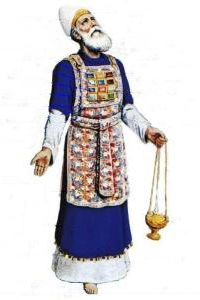
\includegraphics[width=50mm,scale=1.5]{Extras/Melchisedec.jpg}
\vspace{0.4in}  % Create a title for the document and write it in bold font
\LARGE{\textbf{\date}} % Again, do a line break
\linebreak 
% Create a subtitle \large{with Outlines, Statistics, Cross References, and Notes}
\vspace{0.5in}
\begin{flushleft}
\LARGE{Day \#49: Friday, 18 February 2022 PLAIN  \\}\vspace{0.25in}
\LARGE{Numbers 25-27 Psalm 49 Proverb 18}
\end{flushleft}
\vspace{0.6in}
\bigskip

\normalsize{Xenia, Oh.\\}
\normalsize{created: \today}
\vspace{1.3in}

\end{flushright}
\end{titlepage}

\newpage 
\tableofcontents\hypertarget{TOC}{}

\hyphenation{A-bim-e-lech bre-thren E-phra-im  Gib-e-o-nites Jer-u-sa-lem through-out Phil-i-stines The-o-phil-us Am-a-le-kites ven-geance Mesh-el-e-mi-ah onan-ism Phar-a-oh thoughts grev-ous-ness Hach-a-liah adul-ter-er Shad-rach}

%%%%%%%%%%%%%%%%% EXTRA COLORS
%%%%%%%%%%%%%%%%% EXTRA COLORS
%%%%%%%%%%%%%%%%% EXTRA COLORS
\definecolor{champagne}{rgb}{0.97,0.91,0.81}
\definecolor{bone}{rgb}{0.89,0.85,0.79}

\definecolor{ForestGreen}{rgb}{0.00,0.29,0.098}
\definecolor{GIVING}{cmyk}{1,0.0,0.72,.1}

\definecolor{MLPE}{cmyk}{1,1,0,.45}
\definecolor{SOCCER}{cmyk}{.77, 0, .42, .49}
\definecolor{PAYBILL}{cmyk}{0,0.83,0.76,0.07}
\definecolor{SERMON}{cmyk}{.14,.9,0,.30} % aka seance \href{http://www.flatuicolorpicker.com/purple-cmyk-color-model/}{seance}
\definecolor{BIBLE}{cmyk}{0,.17,.74,.17}
\definecolor{WORKBLUE}{cmyk}{1, .5, 0, .6}
\definecolor{myOrange}{cmyk}{0, .4, .98, .03}
\definecolor{myTan}{cmyk}{0.0,.07,.17,.10}
\definecolor{myRed}{cmyk}{0,1,1,0}
\definecolor{myWhite}{cmyk}{0,0,0,0}
\definecolor{BLUESoD}{cmyk}{.97,.84,0,.04}
\definecolor{WHITE}{cmyk}{0,0,0,0}
\definecolor{OLDGOLD}{cmyk}{0.05,0.3,1.00,0}
\definecolor{CASTLETON}{cmyk}{1,0,0.31,0.66}
\definecolor{cadmiumgreen}{rgb}{0.0, 0.42, 0.24}
\definecolor{jungle}{rgb}{0.203,0.4882,0.1718}
\definecolor{MYGOLD}{rgb}{1,.84,0}

\definecolor{MYLIGHTGRAY}{rgb}{.85,.85,.85}

\definecolor{codegreen}{rgb}{0,0.6,0}
\definecolor{codegray}{rgb}{0.5,0.5,0.5}
\definecolor{codepurple}{rgb}{0.58,0,0.82}
\definecolor{backcolour}{rgb}{0.95,0.95,0.92}


\mdfdefinestyle{MyFrame}{%
    linecolor=blue,
    outerlinewidth=2pt,
    roundcorner=5pt,
    innertopmargin=\baselineskip,
    innerbottommargin=\baselineskip,
    innerrightmargin=10pt,
    innerleftmargin=10pt,
    backgroundcolor=gray!25!white}


\mdfdefinestyle{MyFrame2}{%
    linecolor=black,
    outerlinewidth=2pt,
    roundcorner=5pt,
    innertopmargin=\baselineskip,
    innerbottommargin=\baselineskip,
    innerrightmargin=10pt,
    innerleftmargin=10pt,
    backgroundcolor=yellow!25!white}


%%%%%
%% for PFTTIS list
%%%%%

%%% And Joseph said unto
\index[PFTTIS]{And Joseph said unto!Genesis!Gen 40:008}
\index[PFTTIS]{And Joseph said unto!Genesis!Gen 40:012}
\index[PFTTIS]{And Joseph said unto!Genesis!Gen 41:025}
\index[PFTTIS]{And Joseph said unto!Genesis!Gen 42:014}
\index[PFTTIS]{And Joseph said unto!Genesis!Gen 42:018}
\index[PFTTIS]{And Joseph said unto!Genesis!Gen 44:015}
\index[PFTTIS]{And Joseph said unto!Genesis!Gen 45:003}
\index[PFTTIS]{And Joseph said unto!Genesis!Gen 45:004}
\index[PFTTIS]{And Joseph said unto!Genesis!Gen 46:031}
\index[PFTTIS]{And Joseph said unto!Genesis!Gen 48:009}
\index[PFTTIS]{And Joseph said unto!Genesis!Gen 48:018}
\index[PFTTIS]{And Joseph said unto!Genesis!Gen 50:019}
\index[PFTTIS]{And Joseph said unto!Genesis!Gen 50:024}


%%% a shadow
\index[PFTTIS]{a shadow!1Chronicles!1Chr 029:15}
\index[PFTTIS]{a shadow!Job!Job 008:09}
\index[PFTTIS]{a shadow!Job!Job 014:02}
\index[PFTTIS]{a shadow!Job!Job 017:07}
\index[PFTTIS]{a shadow!Psalm!Psa 102:011}
\index[PFTTIS]{a shadow!Psalm!Psa 144:004}
\index[PFTTIS]{a shadow!Ecclesiastes!Eccl 006:012}
\index[PFTTIS]{a shadow!Ecclesiastes!Eccl 008:013}
\index[PFTTIS]{a shadow!Isaiah!Isa 04:006}
\index[PFTTIS]{a shadow!Isaiah!Isa 25:004}
\index[PFTTIS]{a shadow!Jonah!Jnh 04:06}
\index[PFTTIS]{a shadow!Colossians!Col 02:017}
\index[PFTTIS]{a shadow!Hebews!Heb 10:001}

%%% blessed is the man
\index[PFTTIS]{blessed is the man!Psalm!Psa 001:001}
\index[PFTTIS]{blessed is the man!Psalm!Psa 032:002}
\index[PFTTIS]{blessed is the man!Psalm!Psa 034:008}
\index[PFTTIS]{blessed is the man!Psalm!Psa 065:004}
\index[PFTTIS]{blessed is the man!Psalm!Psa 084:005}
\index[PFTTIS]{blessed is the man!Psalm!Psa 084:012}
\index[PFTTIS]{blessed is the man!Psalm!Psa 094:012}
\index[PFTTIS]{blessed is the man!Psalm!Psa 112:001}
\index[PFTTIS]{blessed is the man!Proverbs!Pro 008:034}
\index[PFTTIS]{blessed is the man!Isaiah!Isa 056:002}
\index[PFTTIS]{blessed is the man!Jeremiah!Jer 017:007}
\index[PFTTIS]{blessed is the man!Romans!Rom 004:008}
\index[PFTTIS]{blessed is the man!James!Jam 001:012}


%%% carry them
\index[PFTTIS]{carry them!Leviticus!Lev 14:045}
\index[PFTTIS]{carry them!Numbers!Num 11:012}
\index[PFTTIS]{carry them!Joshua!Jsh 04:003}
\index[PFTTIS]{carry them!1Samuel!1Sam 20:040}
\index[PFTTIS]{carry them!1Kings!1Kng 08:046}
\index[PFTTIS]{carry them!2Chronicles!2Chr 06:036}
\index[PFTTIS]{carry them!Ezra!Ezra 05:015}
\index[PFTTIS]{carry them!Isaiah!Isa 40:011}
\index[PFTTIS]{carry them!Isaiah!Isa 41:016}
\index[PFTTIS]{carry them!Isaiah!Isa 57:013}
\index[PFTTIS]{carry them!Jeremiah!Jer 20:004}
\index[PFTTIS]{carry them!Jeremiah!Jer 20:005}
\index[PFTTIS]{carry them!Jeremiah!Jer 43:012}


\index[PFTTIS]{good tidings!2Samuel!2Sam 18:027}
\index[PFTTIS]{good tidings!1Kings!1Ki 01:042}
\index[PFTTIS]{good tidings!2Kings!2Ki 07:009 (2x)}
\index[PFTTIS]{good tidings!Isaiah!Isa 40:009 (2x)}
\index[PFTTIS]{good tidings!Isaiah!Isa 41:007}
\index[PFTTIS]{good tidings!Isaiah!Isa 52:007}
\index[PFTTIS]{good tidings!Isaiah!Isa 61:001}
\index[PFTTIS]{good tidings!Nahum!Nah 01:005}
\index[PFTTIS]{good tidings!Luke!Lk 02:010}
\index[PFTTIS]{good tidings!1Thessalonians!1Thess 03:006}


%%% dead body
\index[PFTTIS]{dead body!Leviticus!Lev 21:011}
\index[PFTTIS]{dead body!Numbers!Num 06:006}
\index[PFTTIS]{dead body!Numbers!Num 09:006}
\index[PFTTIS]{dead body!Numbers!Num 09:007}
\index[PFTTIS]{dead body!Numbers!Num 09:010}
\index[PFTTIS]{dead body!Numbers!Num 09:011}
\index[PFTTIS]{dead body!Numbers!Num 09:013}
\index[PFTTIS]{dead body!Numbers!Num 09:016}
\index[PFTTIS]{dead body!2Kings!2Ki 08:005}
\index[PFTTIS]{dead body!Isaiah!Isa 26:019}
\index[PFTTIS]{dead body!Jeremiah!Jer 26:023}
\index[PFTTIS]{dead body!Jeremiah!Jer 36:030}
\index[PFTTIS]{dead body!Haggai!Hag 02:013}

%%% great sea
\index[PFTTIS]{great sea!Numbers!Num 34:006}
\index[PFTTIS]{great sea!Numbers!Num 34:007}
\index[PFTTIS]{great sea!Joshua!Jos 01:004}
\index[PFTTIS]{great sea!Joshua!Jos 09:001}
\index[PFTTIS]{great sea!Joshua!Jos 15:012}
\index[PFTTIS]{great sea!Joshua!Jos 15:047}
\index[PFTTIS]{great sea!Joshua!Jos 23:004}
\index[PFTTIS]{great sea!Ezekiel!Eze 47:010}
\index[PFTTIS]{great sea!Ezekiel!Eze 47:015}
\index[PFTTIS]{great sea!Ezekiel!Eze 47:019}
\index[PFTTIS]{great sea!Ezekiel!Eze 47:020}
\index[PFTTIS]{great sea!Ezekiel!Eze 48:028}
\index[PFTTIS]{great sea!Daniel!Dan 07:002}


%%% have forsaken me
\index[PFTTIS]{have forsaken me!Judges!Jdg 10:013}
\index[PFTTIS]{have forsaken me!1Samuel!1Sam 08:008}
\index[PFTTIS]{have forsaken me!1Kings!1Ki 11:033}
\index[PFTTIS]{have forsaken me!2Kings!2Ki 22:017}
\index[PFTTIS]{have forsaken me!2Chronicles!2Chr 12:005}
\index[PFTTIS]{have forsaken me!2Chronicles!2Chr 34:025}
\index[PFTTIS]{have forsaken me!Jeremiah!Jer 01:016}
\index[PFTTIS]{have forsaken me!Jeremiah!Jer 02:013}
\index[PFTTIS]{have forsaken me!Jeremiah!Jer 05:007}
\index[PFTTIS]{have forsaken me!Jeremiah!Jer 05:019}
\index[PFTTIS]{have forsaken me!Jeremiah!Jer 16:011 (2x)}
\index[PFTTIS]{have forsaken me!Jeremiah!Jer 19:004}

%%% no king
\index[PFTTIS]{no king!Judges!Jdg 17:06}
\index[PFTTIS]{no king!Judges!Jdg 18:01}
\index[PFTTIS]{no king!Judges!Jdg 19:01}
\index[PFTTIS]{no king!Judges!Jdg 21:25}
\index[PFTTIS]{no king!1Kings!1Ki 22:47}
\index[PFTTIS]{no king!2Kings!2Ki 23:25}
\index[PFTTIS]{no king!Nehemiah!Neh 13:26}
\index[PFTTIS]{no king!Psalms!Psa 033:016}
\index[PFTTIS]{no king!Proverbs!Pro 30:27}
\index[PFTTIS]{no king!Daniel!Dan 02:10}
\index[PFTTIS]{no king!Hosea!Hos 10:03}
\index[PFTTIS]{no king!Micah!Mic 04:09}
\index[PFTTIS]{no king!John!Jhn 19:15}


%%% rebellious house
\index[PFTTIS]{rebellious house!Exodus!Exo 02:005}
\index[PFTTIS]{rebellious house!Exodus!Exo 02:006}
\index[PFTTIS]{rebellious house!Exodus!Exo 02:008}
\index[PFTTIS]{rebellious house!Exodus!Exo 03:009}
\index[PFTTIS]{rebellious house!Exodus!Exo 03:026}
\index[PFTTIS]{rebellious house!Exodus!Exo 03:027}
\index[PFTTIS]{rebellious house!Exodus!Exo 12:002 (2x)}
\index[PFTTIS]{rebellious house!Exodus!Exo 12:003}
\index[PFTTIS]{rebellious house!Exodus!Exo 12:009}
\index[PFTTIS]{rebellious house!Exodus!Exo 12:025}
\index[PFTTIS]{rebellious house!Exodus!Exo 17:012}
\index[PFTTIS]{rebellious house!Exodus!Exo 24:003}

%%% seek him
\index[PFTTIS]{seek him!Deuteronomy!Deu 04:029}\index[PFTTIS]{seek him!1Samuel!1Sam 23:025}
\index[PFTTIS]{seek him!1Chronicles!1Chr 28:009}
\index[PFTTIS]{seek him!2Chronicles!1Chr 15:002}
\index[PFTTIS]{seek him!Ezra!Ezr 08:022}
\index[PFTTIS]{seek him!Psalms!Psa 022:026}
\index[PFTTIS]{seek him!Psalms!Psa 024:006}
\index[PFTTIS]{seek him!Psalms!Psa 119:002}
\index[PFTTIS]{seek him!SoS!SoS 03:002}
\index[PFTTIS]{seek him!SoS!SoS 06:001}
\index[PFTTIS]{seek him!Hosea!Hos 07:010}
\index[PFTTIS]{seek him!Amos!Amo 05:008}
\index[PFTTIS]{seek him!Hebrews!Heb 11:0063}


%%% seek ye
\index[PFTTIS]{seek ye!Isaiah!Isa 34:016}
\index[PFTTIS]{seek ye!Isaiah!Isa 45:019}
\index[PFTTIS]{seek ye!Isaiah!Isa 55:006}
\index[PFTTIS]{seek ye!Amos!Amos 5:004}
\index[PFTTIS]{seek ye!John!John 1:38}
\index[PFTTIS]{seek ye!John!John 18:4}
\index[PFTTIS]{seek ye!John!John 18:7}
\index[PFTTIS]{seek ye!Matthew!Matt 6:33}
\index[PFTTIS]{seek ye!Numbers!Num 16:10}
\index[PFTTIS]{seek ye!Luke!Luke 12:31}
\index[PFTTIS]{seek ye!Luke!Luke 24:5}
\index[PFTTIS]{seek ye!Psalm!Psa 27:8}
\index[PFTTIS]{seek ye!Zephaniah!Zeph 2:3}

%%% the uncircumcised
\index[PFTTIS]{the uncircumcised!Genesis!Gen 17:014}
\index[PFTTIS]{the uncircumcised!Judges!Jdg 14:003}
\index[PFTTIS]{the uncircumcised!Judges!Jdg 15:018}
\index[PFTTIS]{the uncircumcised!2Samuel!2Sam 01:020}
\index[PFTTIS]{the uncircumcised!Isaiah!Isa 02:001}
\index[PFTTIS]{the uncircumcised!Jeremiah!Jer 09:025}
\index[PFTTIS]{the uncircumcised!Ezekiel!Eze 28:010}
\index[PFTTIS]{the uncircumcised!Ezekiel!Eze 31:018}
\index[PFTTIS]{the uncircumcised!Ezekiel!Eze 32:019}
\index[PFTTIS]{the uncircumcised!Ezekiel!Eze 32:027}
\index[PFTTIS]{the uncircumcised!Ezekiel!Eze 32:028}
\index[PFTTIS]{the uncircumcised!Ezekiel!Eze 32:029}
\index[PFTTIS]{the uncircumcised!Ezekiel!Eze 32:032}

%%% worship him
\index[PFTTIS]{worship him!Psalms!Psa 97:007}
\index[PFTTIS]{worship him!Zephaniah!Zeph 02:011}
\index[PFTTIS]{worship him!Matthew!Matt 02:002}
\index[PFTTIS]{worship him!Matthew!Matt 02:008}
\index[PFTTIS]{worship him!John!John 04:023}
\index[PFTTIS]{worship him!John!John 04:024 (2x)} 
\index[PFTTIS]{worship him!Acts!Acts 17:023}
\index[PFTTIS]{worship him!Hebrews!Heb 01:006}
\index[PFTTIS]{worship him!Revelation!Rev 04:010}
\index[PFTTIS]{worship him!Revelation!Rev 13:008}
\index[PFTTIS]{worship him!Revelation!Rev 14:007}
\index[PFTTIS]{worship him!Revelation!Rev 19:010}


%%%%%
%% for PFTTIS list
%%%%%

%%% afflictions
\index[WFTTIS]{afflictions!Psalms!Psa 34:019}
\index[WFTTIS]{afflictions!Psalms!Psa 132:001}
\index[WFTTIS]{afflictions!Acts!Acts 07:010}
\index[WFTTIS]{afflictions!Acts!Acts 20:023}
\index[WFTTIS]{afflictions!2Corinthians!2Cor 06:004}
\index[WFTTIS]{afflictions!Colossians!Col 01:024}
\index[WFTTIS]{afflictions!1Thessalonians!1Thess 03:003}
\index[WFTTIS]{afflictions!2Timothy!2Tim 01:008}
\index[WFTTIS]{afflictions!2Timothy!2Tim 03:011}
\index[WFTTIS]{afflictions!2Timothy!2Tim 04:005}
\index[WFTTIS]{afflictions!Hebrews!Heb 10:032}
\index[WFTTIS]{afflictions!Hebrews!Heb 10:033}
\index[WFTTIS]{afflictions!1Peter!1Pet 05:009}

%%% acsend
\index[WFTTIS]{acsend!Joshua!Jos 06:05}
\index[WFTTIS]{acsend!Psalm!Psa 024:003}
\index[WFTTIS]{acsend!Psalm!Psa 135:007}
\index[WFTTIS]{acsend!Psalm!Psa 139:008}
\index[WFTTIS]{acsend!Isaiah!Isa 14:013}
\index[WFTTIS]{acsend!Isaiah!Isa 14:014}
\index[WFTTIS]{acsend!Jeremiah!Jer 10:013}
\index[WFTTIS]{acsend!Jeremiah!Jer 51:016}
\index[WFTTIS]{acsend!Ezekiel!Eze 38:009}
\index[WFTTIS]{acsend!John!John 06:062}
\index[WFTTIS]{acsend!John!John 20:017}
\index[WFTTIS]{acsend!Romans!Rom 10:006}
\index[WFTTIS]{acsend!Revelation!Rev 17:008}

%%% Assyrian
\index[WFTTIS]{Assyrian!Isaiah!Isa 10:005}
\index[WFTTIS]{Assyrian!Isaiah!Isa 10:024}
\index[WFTTIS]{Assyrian!Isaiah!Isa 14:025}
\index[WFTTIS]{Assyrian!Isaiah!Isa 19:023}
\index[WFTTIS]{Assyrian!Isaiah!Isa 23:013}
\index[WFTTIS]{Assyrian!Isaiah!Isa 30:031}
\index[WFTTIS]{Assyrian!Isaiah!Isa 31:008}
\index[WFTTIS]{Assyrian!Isaiah!Isa 52:004}
\index[WFTTIS]{Assyrian!Ezekiel!Eze 31:003}
\index[WFTTIS]{Assyrian!Hosea!Hos 05:013}
\index[WFTTIS]{Assyrian!Hosea!Hos 11:005}
\index[WFTTIS]{Assyrian!Micah!Hos 05:005}
\index[WFTTIS]{Assyrian!Micah!Hos 05:006}

%%% blot
\index[WFTTIS]{blot!Exodus!Exo 32:032}
\index[WFTTIS]{blot!Exodus!Exo 32:033}
\index[WFTTIS]{blot!Numbers!Num 05:026}
\index[WFTTIS]{blot!Deuteronomy!Deut 09:014}
\index[WFTTIS]{blot!Deuteronomy!Deut 25:019}
\index[WFTTIS]{blot!Deuteronomy!Deut 29:020}
\index[WFTTIS]{blot!2Kings!2Ki 14:027}
\index[WFTTIS]{blot!Job!Job 31:007}
\index[WFTTIS]{blot!Psalms!Psa 51:001}
\index[WFTTIS]{blot!Psalms!Psa 51:009}
\index[WFTTIS]{blot!Proverbs!Pro 09:007}
\index[WFTTIS]{blot!Jeremiah!Jer 18:023}
\index[WFTTIS]{blot!Revelation!Rev 03:005}


%%% chain
\index[WFTTIS]{chain!Genesis!Gen 41:042}
\index[WFTTIS]{chain!1Kings!1Ki 07:017}
\index[WFTTIS]{chain!Psalms!Psa 73:006}
\index[WFTTIS]{chain!SoS!Sos 04:009}
\index[WFTTIS]{chain!Lamentations!Lam 03:007}
\index[WFTTIS]{chain!Ezekiel!Eze 07:023}
\index[WFTTIS]{chain!Ezekiel!Eze 16:011}
\index[WFTTIS]{chain!Daniel!Dan 05:007}
\index[WFTTIS]{chain!Daniel!Dan 05:016}
\index[WFTTIS]{chain!Daniel!Dan 05:029}
\index[WFTTIS]{chain!Acts!Acts 28:020}
\index[WFTTIS]{chain!2Timothy!2Tim 01:016}
\index[WFTTIS]{chain!Revelation!Rev 20:001}


%%% controversy
\index[WFTTIS]{controversy!Deuteronomy!Deu 17:008}
\index[WFTTIS]{controversy!Deuteronomy!Deu 19:017}
\index[WFTTIS]{controversy!Deuteronomy!Deu 21:005}
\index[WFTTIS]{controversy!Deuteronomy!Deu 25:001}
\index[WFTTIS]{controversy!2Samuel!2Sam 15:002}
\index[WFTTIS]{controversy!Isaiah!Isa 34:008}
\index[WFTTIS]{controversy!Jeremiah!Jer 25:031}
\index[WFTTIS]{controversy!Ezekiel!Eze 44:024}
\index[WFTTIS]{controversy!Hosea!Hos 04:001}
\index[WFTTIS]{controversy!Hosea!Hos 12:002}
\index[WFTTIS]{controversy!Micah!Mic 06:002 (2x)}
\index[WFTTIS]{controversy!1Timothy!1Tim 03:016}


%%% Dagon/Dagon's
\index[WFTTIS]{Dagon!Judges!Jdg 16:023}
\index[WFTTIS]{Dagon!1Samuel!1Sam 05:002 (2x)}
\index[WFTTIS]{Dagon!1Samuel!1Sam 05:003 (2x)}
\index[WFTTIS]{Dagon!1Samuel!1Sam 05:004 (3x)}
\index[WFTTIS]{Dagon!1Samuel!1Sam 05:005 (3x)}
\index[WFTTIS]{Dagon!1Samuel!1Sam 05:007}
\index[WFTTIS]{Dagon!1Chronicles!1Chr 10:010}

%%% disobedient
\index[WFTTIS]{disobedient!1Kings!1Ki 13:026}
\index[WFTTIS]{disobedient!Nehemiah!Neh 09:026}
\index[WFTTIS]{disobedient!Luke!Luke 01:017}
\index[WFTTIS]{disobedient!Acts!Acts 26:019}
\index[WFTTIS]{disobedient!Romans!Rom 01:030}
\index[WFTTIS]{disobedient!Romans!Rom 10:021}
\index[WFTTIS]{disobedient!1Timothy!1Tim 01:009}
\index[WFTTIS]{disobedient!2Timothy!2Tim 03:002}
\index[WFTTIS]{disobedient!Titus!Titus 01:016}
\index[WFTTIS]{disobedient!Titus!Titus 03:003}
\index[WFTTIS]{disobedient!1Peter!1Pet 02:007}
\index[WFTTIS]{disobedient!1Peter!1Pet 02:008}
\index[WFTTIS]{disobedient!1Peter!1Pet 03:020}


%%% doubt
\index[WFTTIS]{doubt!Genesis!Gen 37:033}
\index[WFTTIS]{doubt!Deuteronomy!Deu 28:066}
\index[WFTTIS]{doubt!Job!Job 12:002}
\index[WFTTIS]{doubt!Matthew!Matt 14:031}
\index[WFTTIS]{doubt!Matthew!Matt 21:021}
\index[WFTTIS]{doubt!Mark!Mk 11:023}
\index[WFTTIS]{doubt!Luke!Lk 11:020}
\index[WFTTIS]{doubt!John!Jhn 10:024}
\index[WFTTIS]{doubt!Acts!Acts 02:012}
\index[WFTTIS]{doubt!Acts!Acts 28:004}
\index[WFTTIS]{doubt!1Corinthians!1Cor 09:010}
\index[WFTTIS]{doubt!Galatians!Gal 04:020}
\index[WFTTIS]{doubt!1John!1Jhn 02:019}


%%% dungeon
\index[WFTTIS]{dungeon!Genesis!Gen 40:015}
\index[WFTTIS]{dungeon!Genesis!Gen 41:014}
\index[WFTTIS]{dungeon!Exodus!Exo 12:029}
\index[WFTTIS]{dungeon!Jeremiah!Jer 37:016}
\index[WFTTIS]{dungeon!Jeremiah!Jer 38:006 (2x)}
\index[WFTTIS]{dungeon!Jeremiah!Jer 38:007}
\index[WFTTIS]{dungeon!Jeremiah!Jer 38:009}
\index[WFTTIS]{dungeon!Jeremiah!Jer 38:010}
\index[WFTTIS]{dungeon!Jeremiah!Jer 38:011}
\index[WFTTIS]{dungeon!Jeremiah!Jer 38:013}
\index[WFTTIS]{dungeon!Lamentations!Lam 03:053}
\index[WFTTIS]{dungeon!Lamentations!Lam 03:055}


%%% error
\index[WFTTIS]{error!2Samuel!2Sam 06:007}
\index[WFTTIS]{error!Job!Job 19:004}
\index[WFTTIS]{error!Ecclesiastes!Ecc 05:006}
\index[WFTTIS]{error!Ecclesiastes!Ecc 10:005}
\index[WFTTIS]{error!Isaiah!Isa 32:006}
\index[WFTTIS]{error!Daniel!Dan 06:004}
\index[WFTTIS]{error!Matthew!Matt 27:064}
\index[WFTTIS]{error!Romans!Rom 01:027}
\index[WFTTIS]{error!James!Jam 05:020}
\index[WFTTIS]{error!2Peter!2Pet 02:018}
\index[WFTTIS]{error!2Peter!2Pet 03:017}
\index[WFTTIS]{error!1John!1Jn 04:006}
\index[WFTTIS]{error!Jude!Jude 01:011}

%%% fourish
\index[WFTTIS]{fourish!Psalms!Psa 072:007}
\index[WFTTIS]{fourish!Psalms!Psa 072:016}
\index[WFTTIS]{fourish!Psalms!Psa 092:007}
\index[WFTTIS]{fourish!Psalms!Psa 092:012}
\index[WFTTIS]{fourish!Psalms!Psa 092:013}
\index[WFTTIS]{fourish!Psalms!Psa 132:018}
\index[WFTTIS]{fourish!Proverbs!Pro 11:28}
\index[WFTTIS]{fourish!Proverbs!Pro 14:11}
\index[WFTTIS]{fourish!Ecclesiastes!Ecc 12:05}
\index[WFTTIS]{fourish!SongOfSolomon!SOS 07:12}
\index[WFTTIS]{fourish!Isaiah!Isa 17:11}
\index[WFTTIS]{fourish!Isaiah!Isa 66:14}
\index[WFTTIS]{fourish!Ezekiel!Eze 17:24}




%%% giants
\index[WFTTIS]{giants!Genesis!Gen 06:004}
\index[WFTTIS]{giants!Numbers!Num 13:033}
\index[WFTTIS]{giants!Deuteronomy!Deut 02:011}
\index[WFTTIS]{giants!Deuteronomy!Deut 02:021}
\index[WFTTIS]{giants!Deuteronomy!Deut 03:011}
\index[WFTTIS]{giants!Deuteronomy!Deut 03:013}
\index[WFTTIS]{giants!Joshua!Josh 12:004}
\index[WFTTIS]{giants!Joshua!Josh 13:012}
\index[WFTTIS]{giants!Joshua!Josh 15:008}
\index[WFTTIS]{giants!Joshua!Josh 17:015}
\index[WFTTIS]{giants!Joshua!Josh 16:016}

%%% good man
\index[WFTTIS]{good man!2 Samuel!2Sa 18:27}
%(1) Psalms 37:23 [5]
%(1) Psalms 112:5 [2]
%(1) Proverbs 12:2 [2]
%(1) Proverbs 13:22 [2]
%(1) Proverbs 14:14 [14]
%(1) Micah 7:2 [2]
%(1) Matthew 12:35 [2]
%(1) Luke 6:45 [2]
%(1) Luke 23:50 [15]
%(1) John 7:12 [17]
%(1) Acts 11:24 [5]
%(1) Romans 5:7 [14]

%%% Hinnom
\index[WFTTIS]{Hinnom!Joshua!Jsh 15:008}
\index[WFTTIS]{Hinnom!Joshua!Jsh 18:016}
\index[WFTTIS]{Hinnom!2Kings!2Ki 23:010}
\index[WFTTIS]{Hinnom!2Chronicles!2Chr 28:003}
\index[WFTTIS]{Hinnom!2Chronicles!2Chr 33:006}
\index[WFTTIS]{Hinnom!Nehemiah!Neh 11:030}
\index[WFTTIS]{Hinnom!Jeremiah!Jer 07:031}
\index[WFTTIS]{Hinnom!Jeremiah!Jer 07:032}
\index[WFTTIS]{Hinnom!Jeremiah!Jer 19:002}
\index[WFTTIS]{Hinnom!Jeremiah!Jer 19:006}
\index[WFTTIS]{Hinnom!Jeremiah!Jer 32:035}

%%% inclined
\index[WFTTIS]{inclined!Judges!Jdg 09:003}
\index[WFTTIS]{inclined!Psalms!Psa 040:001}
\index[WFTTIS]{inclined!Psalms!Psa 116:002}
\index[WFTTIS]{inclined!Psalms!Psa 119:112}
\index[WFTTIS]{inclined!Proverbs!Pro 05:13}
\index[WFTTIS]{inclined!Jeremiah!Jer 07:24}
\index[WFTTIS]{inclined!Jeremiah!Jer 07:26}
\index[WFTTIS]{inclined!Jeremiah!Jer 11:08}
\index[WFTTIS]{inclined!Jeremiah!Jer 17:23}
\index[WFTTIS]{inclined!Jeremiah!Jer 25:04}
\index[WFTTIS]{inclined!Jeremiah!Jer 34:14}
\index[WFTTIS]{inclined!Jeremiah!Jer 35:15}
\index[WFTTIS]{inclined!Jeremiah!Jer 44:05}


%%% laughed
\index[WFTTIS]{laughed!Genesis!Gen 17:017}
\index[WFTTIS]{laughed!Genesis!Gen 18:012}
\index[WFTTIS]{laughed!Genesis!Gen 18:015}
\index[WFTTIS]{laughed!2Kings!2Ki 19:021}
\index[WFTTIS]{laughed!2Chronicles!2Chr 30:010}
\index[WFTTIS]{laughed!Nehemiah!Neh 02:019}
\index[WFTTIS]{laughed!Job!Job 12:004}
\index[WFTTIS]{laughed!Job!Job 29:024}
\index[WFTTIS]{laughed!Isaiah!Isa 37:022}
\index[WFTTIS]{laughed!Ezekiel!Ezek 23:032}
\index[WFTTIS]{laughed!Matthew!Matt 09:024}
\index[WFTTIS]{laughed!Mark!Mk 05:040}
\index[WFTTIS]{laughed!Luke!Lk 08:053}

%%% liar
\index[WFTTIS]{liar!Job!Job 24:025}
\index[WFTTIS]{liar!Proverbs!Pro 17:004}
\index[WFTTIS]{liar!Proverbs!Pro 19:022}
\index[WFTTIS]{liar!Proverbs!Pro 30:006}
\index[WFTTIS]{liar!Jeremiah!Jer 15:018}
\index[WFTTIS]{liar!John!Jhn 08:044}
\index[WFTTIS]{liar!John!Jhn 08:055}
\index[WFTTIS]{liar!Romans!Rom 03:004}
\index[WFTTIS]{liar!1John!1Jhn 01:010}
\index[WFTTIS]{liar!1John!1Jhn 02:004}
\index[WFTTIS]{liar!1John!1Jhn 02:022}
\index[WFTTIS]{liar!1John!1Jhn 04:020}
\index[WFTTIS]{liar!1John!1Jhn 05:010}

%%% palsy
\index[WFTTIS]{palsy!Matthew!Matt 04:024}
\index[WFTTIS]{palsy!Matthew!Matt 08:006}
\index[WFTTIS]{palsy!Matthew!Matt 09:002}
\index[WFTTIS]{palsy!Matthew!Matt 09:006}
\index[WFTTIS]{palsy!Mark!Mk 02:003}
\index[WFTTIS]{palsy!Mark!Mk 02:004}
\index[WFTTIS]{palsy!Mark!Mk 02:005}
\index[WFTTIS]{palsy!Mark!Mk 02:009}
\index[WFTTIS]{palsy!Mark!Mk 02:010}
\index[WFTTIS]{palsy!Luke!Lk 05:018}
\index[WFTTIS]{palsy!Luke!Lk 05:024}
\index[WFTTIS]{palsy!Acts!Acts 09:033}

%%% Profitable
\index[WFTTIS]{profitable!Job!Job 22:002 (2x)}
\index[WFTTIS]{profitable!Ecclesiastes!Ecc 10:010}
\index[WFTTIS]{profitable!Isaiah!Isa 44:010}
\index[WFTTIS]{profitable!Jeremiah!Jer 13:007}
\index[WFTTIS]{profitable!Matthew!Matt 05:029}
\index[WFTTIS]{profitable!Matthew!Matt 05:030}
\index[WFTTIS]{profitable!Acts!Acts 20:020}
\index[WFTTIS]{profitable!1Timothy!1Tim 04:008}
\index[WFTTIS]{profitable!2Timothy!2Tim 03:016}
\index[WFTTIS]{profitable!2Timothy!2Tim 04:011}
\index[WFTTIS]{profitable!Titus!Titus 03:008}
\index[WFTTIS]{profitable!Philemon!Phlm 01:011}

%%% Rechab
\index[WFTTIS]{Rechab!2Samuel!2Sam 04:002}
\index[WFTTIS]{Rechab!2Samuel!2Sam 04:005}
\index[WFTTIS]{Rechab!2Samuel!2Sam 04:006}
\index[WFTTIS]{Rechab!2Samuel!2Sam 04:009}
\index[WFTTIS]{Rechab!2KIngs!2Ki 10:015}
\index[WFTTIS]{Rechab!2KIngs!2Ki 10:023}
\index[WFTTIS]{Rechab!1Chronicles!1Chr 02:055}
\index[WFTTIS]{Rechab!Nehemiah!Neh 03:014}
\index[WFTTIS]{Rechab!Jeremiah!Jer 35:006}
\index[WFTTIS]{Rechab!Jeremiah!Jer 35:008}
\index[WFTTIS]{Rechab!Jeremiah!Jer 35:014}
\index[WFTTIS]{Rechab!Jeremiah!Jer 35:016}
\index[WFTTIS]{Rechab!Jeremiah!Jer 35:019}

%%% serpents
\index[WFTTIS]{serpents!Exodus!Exo 07:012}
\index[WFTTIS]{serpents!Numbers!Num 21:006}
\index[WFTTIS]{serpents!Numbers!Num 21:007}
\index[WFTTIS]{serpents!Deuteronomy!Deu 08:015}
\index[WFTTIS]{serpents!Deuteronomy!Deu 32:024}
\index[WFTTIS]{serpents!Jeremiah!Jer 08:017}
\index[WFTTIS]{serpents!Matthew!Matt 10:016}
\index[WFTTIS]{serpents!Matthew!Matt 23:033}
\index[WFTTIS]{serpents!Mark!Mk 16:018}
\index[WFTTIS]{serpents!Luke!Lk 10:019}
\index[WFTTIS]{serpents!1Corinthians!1Cor 10:009}
\index[WFTTIS]{serpents!James!Jas 03:007}
\index[WFTTIS]{serpents!Revelation!Rev 09:019}

%%% short
\index[WFTTIS]{short!Numbers!Num 11:023}
\index[WFTTIS]{short!2Kings!2Ki 10:032}
\index[WFTTIS]{short!Job!Job 17:012}
\index[WFTTIS]{short!Job!Job 20:005}
\index[WFTTIS]{short!Psalms!Psa 89:047}
\index[WFTTIS]{short!Romans!Rom 03:023}
\index[WFTTIS]{short!Romans!Rom 09:028  (2x)}
\index[WFTTIS]{short!1Corinthians!1Cor 07:029}
\index[WFTTIS]{short!1Thessalonians!1Thess 02:017}
\index[WFTTIS]{short!Hebrews!Heb 04:001}
\index[WFTTIS]{short!Revelation!Rev 12:012}
\index[WFTTIS]{short!Revelation!Rev 17:010}

%%% smiteth
\index[WFTTIS]{smiteth!Exodus!Exo 21:012}
\index[WFTTIS]{smiteth!Exodus!Exo 21:15}
\index[WFTTIS]{smiteth!Deuteronomy!Dt 25:11}
\index[WFTTIS]{smiteth!Deuteronomy!Dt 27:24}
\index[WFTTIS]{smiteth!Joshua!Jsh 15:16}
\index[WFTTIS]{smiteth!Judges!Jdg 15:16}
\index[WFTTIS]{smiteth!2 Samuel!2Sa 05:08}
\index[WFTTIS]{smiteth!1Chronicles!1Chr 11:06}
\index[WFTTIS]{smiteth!Job!1Chr 26:12}
\index[WFTTIS]{smiteth!Isaiah!Isa 09:13}
\index[WFTTIS]{smiteth!Lamentations!Lam 03:30}
\index[WFTTIS]{smiteth!Ezekiel!Eze 07:09}
\index[WFTTIS]{smiteth!Luke!Lk 06:29}



%%% vanities
\index[WFTTIS]{vanities!Deuteronomy!Deut 21:021}
\index[WFTTIS]{vanities!1Kings!1Ki 16:013}
\index[WFTTIS]{vanities!1Kings!1Ki 16:026}
\index[WFTTIS]{vanities!Psalms!Psa 031:006}
\index[WFTTIS]{vanities!Ecclesiastes!Ecc 01:002 (2x)}
\index[WFTTIS]{vanities!Ecclesiastes!Ecc 05:007}
\index[WFTTIS]{vanities!Ecclesiastes!Ecc 12:008}
\index[WFTTIS]{vanities!Jeremiah!Jer 08:019}
\index[WFTTIS]{vanities!Jeremiah!Jer 10:008}
\index[WFTTIS]{vanities!Jeremiah!Jer 14:022}
\index[WFTTIS]{vanities!Jonah!Jnh 02:008}
\index[WFTTIS]{vanities!Acts!Acts 14:015}



%%%%%
%% for PFTTIS list
%%%%%

%%% worm
\index[WFITV]{worm!Exodus!Exo 16:024}
\index[WFITV]{worm!Job!Job 17:014}
\index[WFITV]{worm!Job!Job 24:029}
\index[WFITV]{worm!Job!Job 25:005 (2x)}
\index[WFITV]{worm!Psalms!Psa 022:006}
\index[WFITV]{worm!Isaiah!Isa 14:011}
\index[WFITV]{worm!Isaiah!Isa 41:014}
\index[WFITV]{worm!Isaiah!Isa 51:008}
\index[WFITV]{worm!Isaiah!Isa 66:024}
\index[WFITV]{worm!Jonah!Jnh 04:007}
\index[WFITV]{worm!Mark!Mk 09:044}
\index[WFITV]{worm!Mark!Mk 09:046}
\index[WFITV]{worm!Mark!Mk 09:048}


%\subsubsection{Title}
%\textbf{Introduction:} Isaiah 46 
%\index[speaker]{Speaker!Isaiah 49 (Title}
%\index[series]{Book (Speaker)!IPassage (Title)}
%\index[date]{2017/07/09!Isaiah 49 (Title)}
%\begin{compactenum}[I.]
%    \item  \textbf{Point} \index[scripture]{Isaiah!IPassage} (IPassage)
%\end{compactenum}




  


\chapter{Numbers 25}

\begin{figure}
  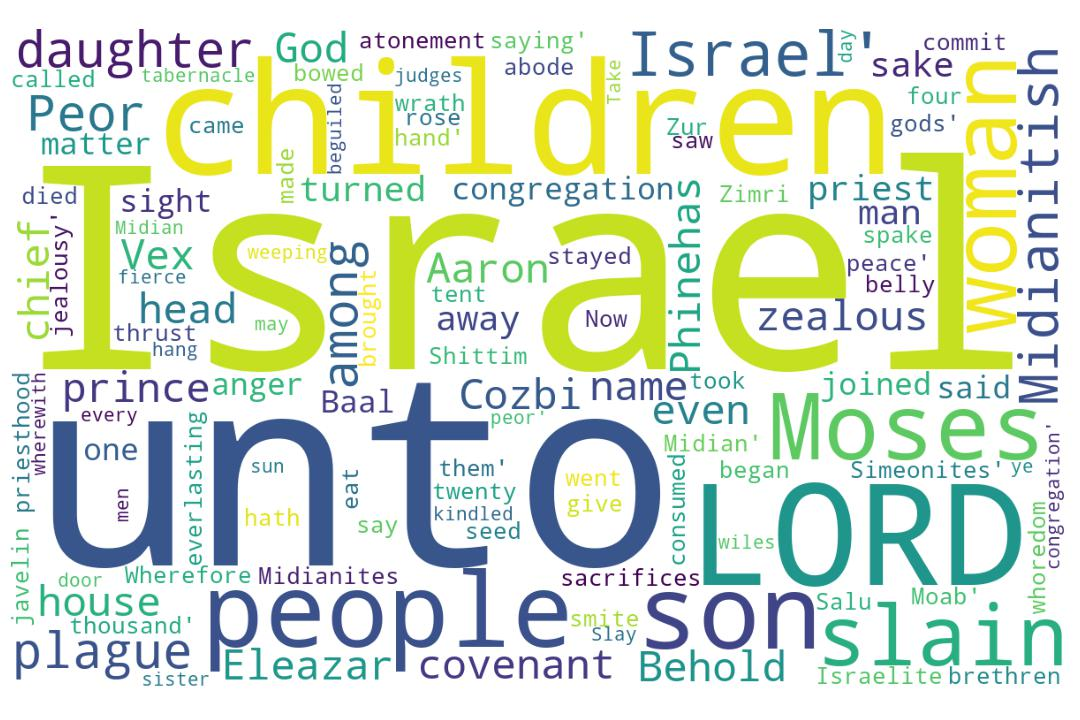
\includegraphics[width=\linewidth]{04OT-Numbers/Numbers25-WordCloud.jpg}
  \caption{Numbers 25 Word Cloud}
  \label{fig:Numbers 25 word Cloud}
\end{figure}

\marginpar{\scriptsize \centering \fcolorbox{bone}{lime}{\textbf{WORSHIP W THE MIDIANITES}}\\ (Numbers 25)
\begin{compactenum}[I.][8]
	\item Go to \textbf{Church} with us \index[scripture]{Numbers!Num 25:02} (Numbers 25:2)
    \item Get \textbf{Carnal} with us \index[scripture]{Numbers!Num 25:02} (Numbers 25:2)
    \item Get \textbf{Corrupted} with us \index[scripture]{Numbers!Num 25:02} (Numbers 25:2)
    \item Get \textbf{Condemned} with us \index[scripture]{Numbers!Num 25:02} (Numbers 25:2)
    \item Get \textbf{Corrected} without us \index[scripture]{Numbers!Num 25:04} (Numbers 25:4)
    \item Get \textbf{Cleansed} within us \index[scripture]{Numbers!Num 25:07} (Numbers 25:7)
\end{compactenum}}

\marginpar{\scriptsize \centering \fcolorbox{bone}{yellow}{\textbf{MAKING A POINT}}\\ (Numbers 25)
\begin{compactenum}[I.][8]
    \item The \textbf{Midianite Prince} with us \index[scripture]{Numbers!Num 25:15} (Numbers 25:15)
    \item The \textbf{Midianite Problem} \index[scripture]{Numbers!Num 25:13} (Numbers 25:13)
    \item A \textbf{Motivated Priest} \index[scripture]{Numbers!Num 25:06} (Numbers 25:6)
    \item A \textbf{Mighty Passion} \index[scripture]{Numbers!Num 25:13} (Numbers 25:13)
    \item A \textbf{Majestic Promise} \index[scripture]{Numbers!Num 25:13} (Numbers 25:13)
    \item This \textbf{Man Phineas} \index[scripture]{Numbers!Num 25:07} (Numbers 25:7)
\end{compactenum}}

%%%%%%%%%%%%%%%%%%%%%%%%%%%%%%%%%%
%%%%%%%%%%%%%%%%%%%%%%%%%%%%%%%%%%
\footnote{\textcolor[rgb]{0.00,0.25,0.00}{\hyperlink{TOC}{Return to end of Table of Contents.}}}\footnote{\href{https://audiobible.com/bible/numbers_25.html}{\textcolor[cmyk]{0.99998,1,0,0}{Numbers 25 Audio}}}\textcolor[cmyk]{0.99998,1,0,0}{\fcolorbox{bone}{bone}{And} \fcolorbox{bone}{bone}{Israel} abode in Shittim, and the people began to commit whoredom with the daughters of Moab.}
[2] \textcolor[cmyk]{0.99998,1,0,0}{\fcolorbox{bone}{bone}{And} they called the people unto the sacrifices of their gods: and the people did eat, and bowed down to their gods.}
[3] \textcolor[cmyk]{0.99998,1,0,0}{\fcolorbox{bone}{bone}{And} \fcolorbox{bone}{bone}{Israel} joined himself unto Baal-peor: and the anger of the LORD was kindled against \fcolorbox{bone}{bone}{Israel}.}
[4] \textcolor[cmyk]{0.99998,1,0,0}{\fcolorbox{bone}{bone}{And} the LORD said unto Moses, Take all the heads of the people, and hang them up before the LORD against the sun, that the fierce anger of the LORD may be turned away from \fcolorbox{bone}{bone}{Israel}.}
[5] \textcolor[cmyk]{0.99998,1,0,0}{\fcolorbox{bone}{bone}{And} Moses said unto the judges of \fcolorbox{bone}{bone}{Israel}, Slay ye every one his men that were joined unto Baal-peor.}\\
\\
\P \textcolor[cmyk]{0.99998,1,0,0}{\fcolorbox{bone}{bone}{And}, behold, one of the children of \fcolorbox{bone}{bone}{Israel} came and brought unto his brethren a Midianitish woman in the sight of Moses, and in the sight of all the congregation of the children of \fcolorbox{bone}{bone}{Israel}, who \emph{were} weeping \emph{before} the door of the tabernacle of the congregation.}
[7] \textcolor[cmyk]{0.99998,1,0,0}{\fcolorbox{bone}{bone}{And} when Phinehas, the son of Eleazar, the son of Aaron the priest, saw \emph{it}, he rose up from among the congregation, and took a javelin in his hand;}
[8] \textcolor[cmyk]{0.99998,1,0,0}{\fcolorbox{bone}{bone}{And} he went after the man of \fcolorbox{bone}{bone}{Israel} into the tent, and thrust both of them through, the man of \fcolorbox{bone}{bone}{Israel}, and the woman through her belly. So the plague was stayed from the children of \fcolorbox{bone}{bone}{Israel}.}
[9] \textcolor[cmyk]{0.99998,1,0,0}{\fcolorbox{bone}{bone}{And} those that died in the plague were twenty and four thousand.}\\
\\
\P  \textcolor[cmyk]{0.99998,1,0,0}{\fcolorbox{bone}{bone}{And} the LORD spake unto Moses, saying,}
[11] \textcolor[cmyk]{0.99998,1,0,0}{Phinehas, the son of Eleazar, the son of Aaron the priest, hath turned my wrath away from the children of \fcolorbox{bone}{bone}{Israel}, while he was zealous for my sake among them, that I consumed not the children of \fcolorbox{bone}{bone}{Israel} in my jealousy.}
[12] \textcolor[cmyk]{0.99998,1,0,0}{Wherefore say, Behold, I give unto him my covenant of peace:}
[13] \textcolor[cmyk]{0.99998,1,0,0}{\fcolorbox{bone}{bone}{And} he shall have it, and his seed after him, \emph{even} the covenant of an everlasting priesthood; because he was zealous for his God, and made an atonement for the children of \fcolorbox{bone}{bone}{Israel}.}
[14] \textcolor[cmyk]{0.99998,1,0,0}{Now the name of the Israelite that was slain, \emph{even} that was slain with the Midianitish woman, \emph{was} Zimri, the son of Salu, a prince of a chief house among the Simeonites.}
[15] \textcolor[cmyk]{0.99998,1,0,0}{\fcolorbox{bone}{bone}{And} the name of the Midianitish woman that was slain \emph{was} Cozbi, the daughter of Zur; he \emph{was} head over a people, \emph{and} of a chief house in Midian.}\\
\\
\P \textcolor[cmyk]{0.99998,1,0,0}{\fcolorbox{bone}{bone}{And} the LORD spake unto Moses, saying,}
[17] \textcolor[cmyk]{0.99998,1,0,0}{Vex the Midianites, and smite them:}
[18] \textcolor[cmyk]{0.99998,1,0,0}{For they vex you with their wiles, wherewith they have beguiled you in the matter of Peor, and in the matter of Cozbi, the daughter of a prince of Midian, their sister, which was slain in the day of the plague for Peor's sake.}
\chapter{Numbers 26}

\begin{figure}
  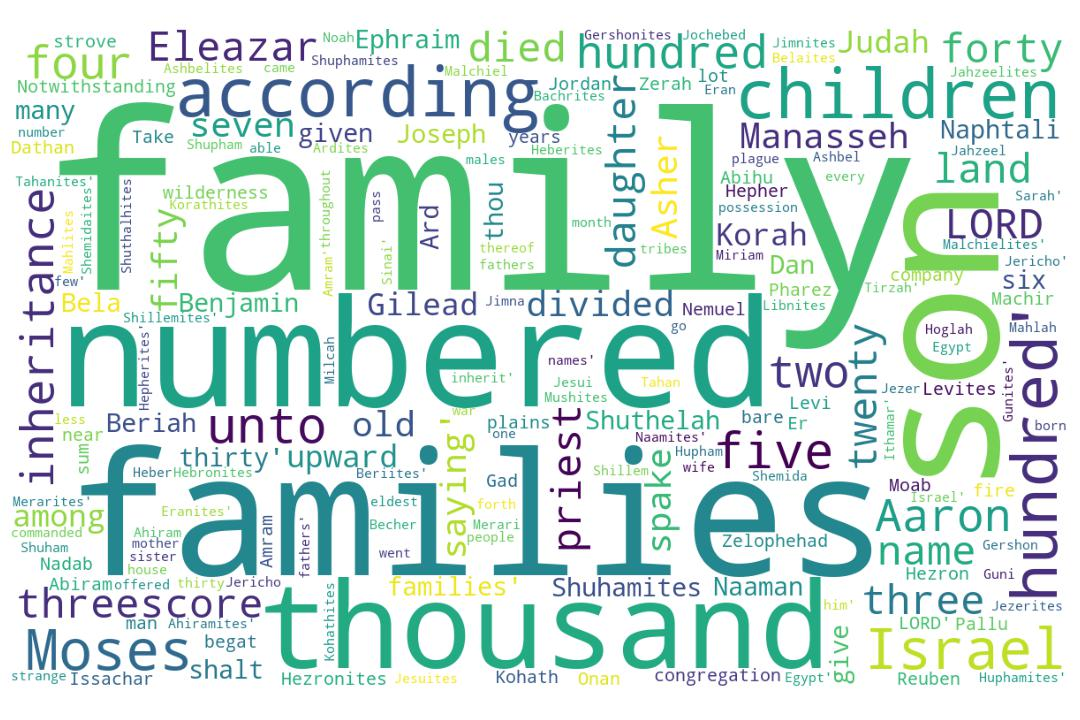
\includegraphics[width=\linewidth]{04OT-Numbers/Numbers26-WordCloud.jpg}
  \caption{Numbers 26 Word Cloud}
  \label{fig:Numbers 26 word Cloud}
\end{figure}

\marginpar{\scriptsize \centering \fcolorbox{bone}{lime}{\textbf{A GENERATION LATER}}\\ (Numbers 26)
\begin{compactenum}[I.][8]
    \item The \textbf{Priests} \index[scripture]{Numbers!Num 26:01}\index[scripture]{Numbers!Num 26:03}\index[scripture]{Numbers!Num 26:63}\index[scripture]{Numbers!Num 26:64} (Numbers 26:1, 3, 63, 64)
    \item The \textbf{Plague} \index[scripture]{Numbers!Num 26:01} (Numbers 26:1)
    \item The \textbf{Plains} of Moab \index[scripture]{Numbers!Num 26:03}\index[scripture]{Numbers!Num 26:64} (Numbers 26:3, 64)
    \item The \textbf{People} 
    \item The \textbf{Population} \index[scripture]{Numbers!Num 26:12--54} (Numbers 26:12--54) Note the differences in population among the various tribes. Simeon loses almost 63\% of its people, while some of the tribes grow substantially.
    \item The \textbf{Possessions} \index[scripture]{Numbers!Num 26:56} (Numbers 26:56)
    \item A \textbf{Preview} 
\end{compactenum}}

%%%%%%%%%%%%%%%%%%%%%%%%%%%%%%%%%%
%%%%%%%%%%%%%%%%%%%%%%%%%%%%%%%%%%
\footnote{\textcolor[rgb]{0.00,0.25,0.00}{\hyperlink{TOC}{Return to end of Table of Contents.}}}\footnote{\href{https://audiobible.com/bible/numbers_26.html}{\textcolor[cmyk]{0.99998,1,0,0}{Numbers 26 Audio}}}\textcolor[cmyk]{0.99998,1,0,0}{And it came to pass after the plague, that the LORD spake unto Moses and unto Eleazar the son of Aaron the priest, saying,}
[2] \textcolor[cmyk]{0.99998,1,0,0}{Take the sum of all the congregation of the children of Israel, from twenty years old and upward, throughout their fathers' house, all that are able to go to war in Israel.}
[3] \textcolor[cmyk]{0.99998,1,0,0}{And Moses and Eleazar the priest spake with them in the plains of Moab by Jordan \emph{near} Jericho, saying,}
[4] \textcolor[cmyk]{0.99998,1,0,0}{\emph{Take} \emph{the} \emph{sum} \emph{of} \emph{the} \emph{people}, from twenty years old and upward; as the LORD commanded Moses and the children of Israel, which went forth out of the land of Egypt.}\\
\\
\P \textcolor[cmyk]{0.99998,1,0,0}{Reuben, the eldest son of Israel: the children of Reuben; Hanoch, \emph{of} \emph{whom} \emph{cometh} the family of the Hanochites: of Pallu, the family of the Palluites:}
[6] \textcolor[cmyk]{0.99998,1,0,0}{Of Hezron, the family of the Hezronites: of Carmi, the family of the Carmites.}
[7] \textcolor[cmyk]{0.99998,1,0,0}{These \emph{are} \fcolorbox{bone}{bone}{the familes} of the Reubenites: and they that were numbered of them were forty and three \fcolorbox{bone}{bone}{thousand and} seven hundred and thirty.}
[8] \textcolor[cmyk]{0.99998,1,0,0}{And the sons of Pallu; Eliab.}
[9] \textcolor[cmyk]{0.99998,1,0,0}{And the sons of Eliab; Nemuel, and Dathan, and Abiram. This \emph{is} \emph{that} Dathan and Abiram, \emph{which} \emph{were} famous in the congregation, who strove against Moses and against Aaron in the company of Korah, when they strove against the LORD:}\footnote{\textbf{Numbers 16:1-3} - Now Korah, the son of Izhar, the son of Kohath, the son of Levi, and Dathan and Abiram, the sons of Eliab, and On, the son of Peleth, sons of Reuben, took men: [2] And they rose up before Moses, with certain of the children of Israel, two hundred and fifty princes of the assembly, famous in the congregation, men of renown: [3] And they gathered themselves together against Moses and against Aaron, and said unto them, Ye take too much upon you, seeing all the congregation are holy, every one of them, and the LORD is among them: wherefore then lift ye up yourselves above the congregation of the LORD?}\footnote{\textbf{Deuteronomy 11:6} - And what he did unto Dathan and Abiram, the sons of Eliab, the son of Reuben: how the earth opened her mouth, and swallowed them up, and their households, and their tents, and all the substance that was in their possession, in the midst of all Israel:}\footnote{\textbf{Psalm 106:17} - The earth opened and swallowed up Dathan, and covered the company of Abiram.}
[10] \textcolor[cmyk]{0.99998,1,0,0}{And the earth opened her mouth, and swallowed them up together with Korah, when that company died, what time the fire devoured two hundred and fifty men: and they became a sign.}
[11] \textcolor[cmyk]{0.99998,1,0,0}{Notwithstanding the children of Korah died not.}\\
\\
\P \textcolor[cmyk]{0.99998,1,0,0}{The sons of Simeon after their families: of Nemuel, the family of the Nemuelites: of Jamin, the family of the Jaminites: of Jachin, the family of the Jachinites:}
[13] \textcolor[cmyk]{0.99998,1,0,0}{Of Zerah, the family of the Zarhites: of Shaul, the family of the Shaulites.}
[14] \textcolor[cmyk]{0.99998,1,0,0}{These \emph{are} \fcolorbox{bone}{bone}{the familes} of the Simeonites, twenty and two \fcolorbox{bone}{bone}{thousand and} two hundred.}\\
\\
\P \textcolor[cmyk]{0.99998,1,0,0}{The children of Gad after their families: of Zephon, the family of the Zephonites: of Haggi, the family of the Haggites: of Shuni, the family of the Shunites:}
[16] \textcolor[cmyk]{0.99998,1,0,0}{Of Ozni, the family of the Oznites: of Eri, the family of the Erites:}
[17] \textcolor[cmyk]{0.99998,1,0,0}{Of Arod, the family of the Arodites: of Areli, the family of the Arelites.}
[18] \textcolor[cmyk]{0.99998,1,0,0}{These \emph{are} \fcolorbox{bone}{bone}{the familes} of the children of Gad according to those that were numbered of them, forty \fcolorbox{bone}{bone}{thousand and} five hundred.}\\
\\
\P \textcolor[cmyk]{0.99998,1,0,0}{The sons of Judah \emph{were} Er and Onan: and Er and Onan died in the land of Canaan.}
[20] \textcolor[cmyk]{0.99998,1,0,0}{And the sons of Judah after their families were; of Shelah, the family of the Shelanites: of Pharez, the family of the Pharzites: of Zerah, the family of the Zarhites.}
[21] \textcolor[cmyk]{0.99998,1,0,0}{And the sons of Pharez were; of Hezron, the family of the Hezronites: of Hamul, the family of the Hamulites.}
[22] \textcolor[cmyk]{0.99998,1,0,0}{These \emph{are} \fcolorbox{bone}{bone}{the familes} of Judah according to those that were numbered of them, threescore and sixteen \fcolorbox{bone}{bone}{thousand and} five hundred.}\\
\\
\P \textcolor[cmyk]{0.99998,1,0,0}{\emph{Of} the sons of Issachar after their families: \emph{of} Tola, the family of the Tolaites: of Pua, the family of the Punites:}
[24] \textcolor[cmyk]{0.99998,1,0,0}{Of Jashub, the family of the Jashubites: of Shimron, the family of the Shimronites.}
[25] \textcolor[cmyk]{0.99998,1,0,0}{These \emph{are} \fcolorbox{bone}{bone}{the familes} of Issachar according to those that were numbered of them, threescore and four \fcolorbox{bone}{bone}{thousand and} three hundred.}\\
\\
\P \textcolor[cmyk]{0.99998,1,0,0}{\emph{Of} the sons of Zebulun after their families: of Sered, the family of the Sardites: of Elon, the family of the Elonites: of Jahleel, the family of the Jahleelites.}
[27] \textcolor[cmyk]{0.99998,1,0,0}{These \emph{are} \fcolorbox{bone}{bone}{the familes} of the Zebulunites according to those that were numbered of them, threescore \fcolorbox{bone}{bone}{thousand and} five hundred.}\\
\\
\P \textcolor[cmyk]{0.99998,1,0,0}{The sons of Joseph after their families \emph{were} Manasseh and Ephraim.}
[29] \textcolor[cmyk]{0.99998,1,0,0}{Of the sons of Manasseh: of Machir, the family of the Machirites: and Machir begat Gilead: of Gilead \emph{come} the family of the Gileadites.}
[30] \textcolor[cmyk]{0.99998,1,0,0}{These \emph{are} the sons of Gilead: \emph{of} Jeezer, the family of the Jeezerites: of Helek, the family of the Helekites:}
[31] \textcolor[cmyk]{0.99998,1,0,0}{And \emph{of} Asriel, the family of the Asrielites: and \emph{of} Shechem, the family of the Shechemites:}
[32] \textcolor[cmyk]{0.99998,1,0,0}{And \emph{of} Shemida, the family of the Shemidaites: and \emph{of} Hepher, the family of the Hepherites.}
[33] \textcolor[cmyk]{0.99998,1,0,0}{And Zelophehad the son of Hepher had no sons, but daughters: and the names of the daughters of Zelophehad \emph{were} Mahlah, and Noah, Hoglah, Milcah, and Tirzah.}
[34] \textcolor[cmyk]{0.99998,1,0,0}{These \emph{are} \fcolorbox{bone}{bone}{the familes} of Manasseh, and those that were numbered of them, fifty and two \fcolorbox{bone}{bone}{thousand and} seven hundred.}\\
\\
\P \textcolor[cmyk]{0.99998,1,0,0}{These \emph{are} the sons of Ephraim after their families: of Shuthelah, the family of the Shuthalhites: of Becher, the family of the Bachrites: of Tahan, the family of the Tahanites.}
[36] \textcolor[cmyk]{0.99998,1,0,0}{And these \emph{are} the sons of Shuthelah: of Eran, the family of the Eranites.}
[37] \textcolor[cmyk]{0.99998,1,0,0}{These \emph{are} \fcolorbox{bone}{bone}{the familes} of the sons of Ephraim according to those that were numbered of them, thirty and two \fcolorbox{bone}{bone}{thousand and} five hundred. These \emph{are} the sons of Joseph after their families.}\\
\\
\P \textcolor[cmyk]{0.99998,1,0,0}{The sons of Benjamin after their families: of Bela, the family of the Belaites: of Ashbel, the family of the Ashbelites: of Ahiram, the family of the Ahiramites:}
[39] \textcolor[cmyk]{0.99998,1,0,0}{Of Shupham, the family of the Shuphamites: of Hupham, the family of the Huphamites.}
[40] \textcolor[cmyk]{0.99998,1,0,0}{And the sons of Bela were Ard and Naaman: \emph{of} \emph{Ard}, the family of the Ardites: \emph{and} of Naaman, the family of the Naamites.}
[41] \textcolor[cmyk]{0.99998,1,0,0}{These \emph{are} the sons of Benjamin after their families: and they that were numbered of them \emph{were} forty and five \fcolorbox{bone}{bone}{thousand and} six hundred.}\\
\\
\P \textcolor[cmyk]{0.99998,1,0,0}{These \emph{are} the sons of Dan after their families: of Shuham, the family of the Shuhamites. These \emph{are} \fcolorbox{bone}{bone}{the familes} of Dan after their families.}
[43] \textcolor[cmyk]{0.99998,1,0,0}{All \fcolorbox{bone}{bone}{the familes} of the Shuhamites, according to those that were numbered of them, \emph{were} threescore and four \fcolorbox{bone}{bone}{thousand and} four hundred.}\\
\\
\P \textcolor[cmyk]{0.99998,1,0,0}{\emph{Of} the children of Asher after their families: of Jimna, the family of the Jimnites: of Jesui, the family of the Jesuites: of Beriah, the family of the Beriites.}
[45] \textcolor[cmyk]{0.99998,1,0,0}{Of the sons of Beriah: of Heber, the family of the Heberites: of Malchiel, the family of the Malchielites.}
[46] \textcolor[cmyk]{0.99998,1,0,0}{And the name of the daughter of Asher \emph{was} Sarah.}
[47] \textcolor[cmyk]{0.99998,1,0,0}{These \emph{are} \fcolorbox{bone}{bone}{the familes} of the sons of Asher according to those that were numbered of them; \emph{who} \emph{were} fifty and three \fcolorbox{bone}{bone}{thousand and} four hundred.}\\
\\
\P \textcolor[cmyk]{0.99998,1,0,0}{\emph{Of} the sons of Naphtali after their families: of Jahzeel, the family of the Jahzeelites: of Guni, the family of the Gunites:}
[49] \textcolor[cmyk]{0.99998,1,0,0}{Of Jezer, the family of the Jezerites: of Shillem, the family of the Shillemites.}
[50] \textcolor[cmyk]{0.99998,1,0,0}{These \emph{are} \fcolorbox{bone}{bone}{the familes} of Naphtali according to their families: and they that were numbered of them \emph{were} forty and five \fcolorbox{bone}{bone}{thousand and} four hundred.}
[51] \textcolor[cmyk]{0.99998,1,0,0}{These \emph{were} the numbered of the children of Israel, six hundred \fcolorbox{bone}{bone}{thousand and} a thousand seven hundred and thirty.}\\
\\
\P \textcolor[cmyk]{0.99998,1,0,0}{And the LORD spake unto Moses, saying,}
[53] \textcolor[cmyk]{0.99998,1,0,0}{Unto these the land shall be divided for an inheritance according to the number of names.}
[54] \textcolor[cmyk]{0.99998,1,0,0}{To many thou shalt give the more inheritance, and to few thou shalt give the less inheritance: to every one shall his inheritance be given according to those that were numbered of him.}
[55] \textcolor[cmyk]{0.99998,1,0,0}{Notwithstanding the land shall be divided by lot: according to the names of the tribes of their fathers they shall inherit.}
[56] \textcolor[cmyk]{0.99998,1,0,0}{According to the lot shall the possession thereof be divided between many and few.}\\
\\
\P \textcolor[cmyk]{0.99998,1,0,0}{And these \emph{are} they that were numbered of the Levites after their families: of Gershon, the family of the Gershonites: of Kohath, the family of the Kohathites: of Merari, the family of the Merarites.}
[58] \textcolor[cmyk]{0.99998,1,0,0}{These \emph{are} \fcolorbox{bone}{bone}{the familes} of the Levites: the family of the Libnites, the family of the Hebronites, the family of the Mahlites, the family of the Mushites, the family of the Korathites. And Kohath begat Amram.}
[59] \textcolor[cmyk]{0.99998,1,0,0}{And the name of Amram's wife \emph{was} Jochebed, the daughter of Levi, whom \emph{her} \emph{mother} bare to Levi in Egypt: and she bare unto Amram Aaron and Moses, and Miriam their sister.}
[60] \textcolor[cmyk]{0.99998,1,0,0}{And unto Aaron was born Nadab, and Abihu, Eleazar, and Ithamar.}
[61] \textcolor[cmyk]{0.99998,1,0,0}{And Nadab and Abihu died, when they offered strange fire before the LORD.}\footnote{\textbf{Numbers 3:4} - And Nadab and Abihu died before the LORD, when they offered strange fire before the LORD, in the wilderness of Sinai, and they had no children: and Eleazar and Ithamar ministered in the priest’s office in the sight of Aaron their father.}\footnote{\textbf{Numbers 10:1-2} - And Nadab and Abihu, the sons of Aaron, took either of them his censer, and put fire therein, and put incense thereon, and offered strange fire before the LORD, which he commanded them not. [2] And there went out fire from the LORD, and devoured them, and they died before the LORD.}
[62] \textcolor[cmyk]{0.99998,1,0,0}{And those that were numbered of them were twenty and three thousand, all males from a month old and upward: for they were not numbered among the children of Israel, because there was no inheritance given them among the children of Israel.}
[63] \textcolor[cmyk]{0.99998,1,0,0}{These \emph{are} they that were numbered by Moses and Eleazar the priest, who numbered the children of Israel in the plains of Moab by Jordan \emph{near} Jericho.}
[64] \textcolor[cmyk]{0.99998,1,0,0}{But among these there was not a man of them whom Moses and Aaron the priest numbered, when they numbered the children of Israel in the wilderness of Sinai.}
[65] \textcolor[cmyk]{0.99998,1,0,0}{For the LORD had said of them, They shall surely die in the wilderness. And there was not left a man of them, save Caleb the son of Jephunneh, and Joshua the son of Nun.}
\chapter{Numbers 27}

\begin{figure}
  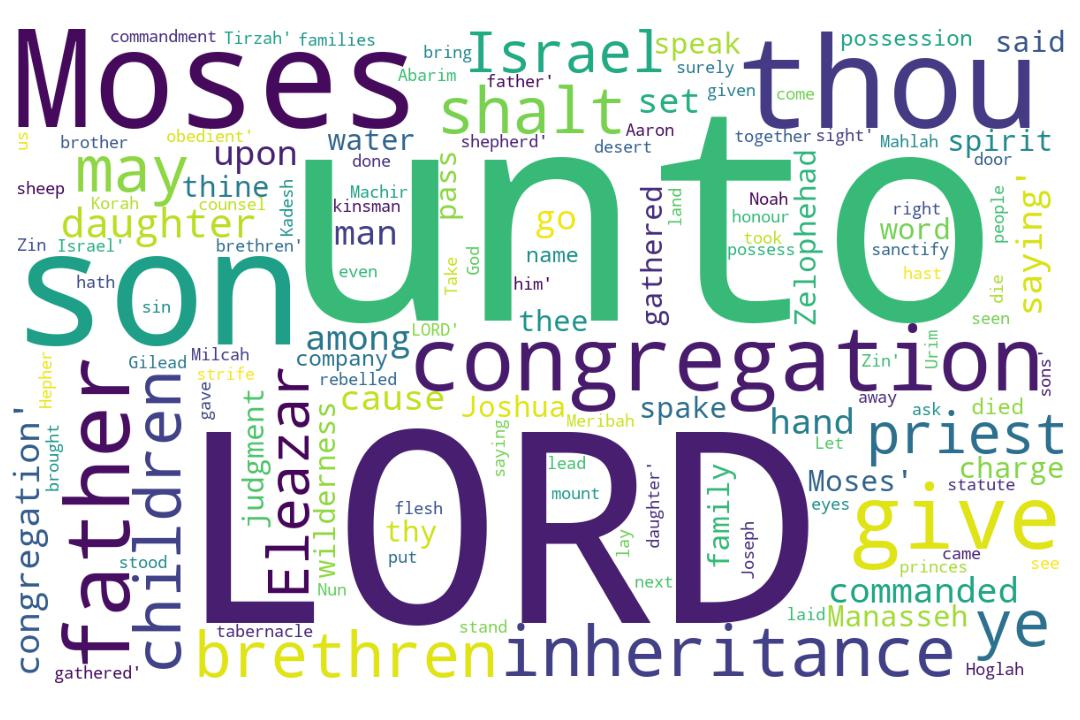
\includegraphics[width=\linewidth]{04OT-Numbers/Numbers27-WordCloud.jpg}
  \caption{Numbers 27 Word Cloud}
  \label{fig:Numbers 27 word Cloud}
\end{figure}

\marginpar{\scriptsize \centering \fcolorbox{blue}{lime}{\textbf{DAUGHTERS OF ZELOPHEHAD}}\\ (Numbers 27)
\begin{compactenum}[I.][8]
    \item \textbf{Single and Dispossessed} \index[scripture]{Numbers!Num 27:01--04} (Numbers 27:2--4)
    \item \textbf{Standing  before the Priests} \index[scripture]{Numbers!Num 27:02} (Numbers 27:2)
    \item A \textbf{Significant Problems} \index[scripture]{Numbers!Num 27:04} (Numbers 27:4)
    \item A \textbf{Sought Possession} \index[scripture]{Numbers!Num 27:04} (Numbers 27:4)
    \item The \textbf{Stated Plan} \index[scripture]{Numbers!Num 27:08--10} (Numbers 27:8--10)
\end{compactenum}}

%%%%%%%%%%%%%%%%%%%%%%%%%%%%%%%%%%
%%%%%%%%%%%%%%%%%%%%%%%%%%%%%%%%%%
\footnote{\textcolor[rgb]{0.00,0.25,0.00}{\hyperlink{TOC}{Return to end of Table of Contents.}}}\footnote{\href{https://audiobible.com/bible/numbers_27.html}{\textcolor[cmyk]{0.99998,1,0,0}{Numbers 27 Audio}}}\textcolor[cmyk]{0.99998,1,0,0}{Then came the daughters of Zelophehad, the son of Hepher, the son of Gilead, the son of Machir, the son of Manasseh, of the families of Manasseh the son of Joseph: and these \emph{are} the names of his daughters; Mahlah, Noah, and Hoglah, and Milcah, and Tirzah.}
[2] \textcolor[cmyk]{0.99998,1,0,0}{And they stood \fcolorbox{bone}{bone}{before} Moses, and \fcolorbox{bone}{bone}{before} Eleazar the priest, and \fcolorbox{bone}{bone}{before} the princes and all the congregation, \emph{by} the door of the tabernacle of the congregation, saying,}
[3] \textcolor[cmyk]{0.99998,1,0,0}{Our father died \fcolorbox{bone}{bone}{in} the wilderness, and he was not \fcolorbox{bone}{bone}{in} the company of them that gathered themselves together against the LORD \fcolorbox{bone}{bone}{in} the company of Korah; but died \fcolorbox{bone}{bone}{in} his own sin, and had no sons.}
[4] \textcolor[cmyk]{0.99998,1,0,0}{Why should the name of our father be done away from among his family, because he hath no son? Give unto us \emph{therefore} a possession among the brethren of our father.}
[5] \textcolor[cmyk]{0.99998,1,0,0}{And Moses brought their cause \fcolorbox{bone}{bone}{before} the LORD.}\\
\\
\P \textcolor[cmyk]{0.99998,1,0,0}{And the LORD spake unto Moses, saying,}
[7] \textcolor[cmyk]{0.99998,1,0,0}{The daughters of Zelophehad speak right: thou shalt surely give them a possession of an inheritance among their father's brethren; and thou shalt cause the inheritance of their father to pass unto them.}
[8] \textcolor[cmyk]{0.99998,1,0,0}{And thou shalt speak unto the children of Israel, saying, If a man die, and have no son, then ye shall cause his inheritance to pass unto his daughter.}
[9] \textcolor[cmyk]{0.99998,1,0,0}{And if he have no daughter, then ye shall give his inheritance unto his brethren.}
[10] \textcolor[cmyk]{0.99998,1,0,0}{And if he have no brethren, then ye shall give his inheritance unto his father's brethren.}
[11] \textcolor[cmyk]{0.99998,1,0,0}{And if his father have no brethren, then ye shall give his inheritance unto his kinsman that is next to him of his family, and he shall possess it: and it shall be unto the children of Israel a statute of judgment, as the LORD commanded Moses.}\\
\\
\P \textcolor[cmyk]{0.99998,1,0,0}{And the LORD said unto Moses, Get thee up into this mount Abarim, and see the land which I have given unto the children of Israel.}
[13] \textcolor[cmyk]{0.99998,1,0,0}{And when thou hast seen it, thou also shalt be gathered unto thy people, as Aaron thy brother was gathered.}
[14] \textcolor[cmyk]{0.99998,1,0,0}{For ye rebelled against my commandment \fcolorbox{bone}{bone}{in} the desert of Zin, \fcolorbox{bone}{bone}{in} the strife of the congregation, to sanctify me at the water \fcolorbox{bone}{bone}{before} their eyes: that \emph{is} the water of Meribah \fcolorbox{bone}{bone}{in} Kadesh \fcolorbox{bone}{bone}{in} the wilderness of Zin.}\\
\\
\P \textcolor[cmyk]{0.99998,1,0,0}{And Moses spake unto the LORD, saying,}
[16] \textcolor[cmyk]{0.99998,1,0,0}{Let the LORD, the God of the spirits of all flesh, set a man over the congregation,}
[17] \textcolor[cmyk]{0.99998,1,0,0}{Which may go out \fcolorbox{bone}{bone}{before} them, and which may go \fcolorbox{bone}{bone}{in} \fcolorbox{bone}{bone}{before} them, and which may lead them out, and which may bring them \fcolorbox{bone}{bone}{in}; that the congregation of the LORD be not as sheep which have no shepherd.}\\
\\
\P \textcolor[cmyk]{0.99998,1,0,0}{And the LORD said unto Moses, Take thee Joshua the son of Nun, a man \fcolorbox{bone}{bone}{in} whom \emph{is} the spirit, and lay thine hand upon him;}
[19] \textcolor[cmyk]{0.99998,1,0,0}{And set him \fcolorbox{bone}{bone}{before} Eleazar the priest, and \fcolorbox{bone}{bone}{before} all the congregation; and give him a charge \fcolorbox{bone}{bone}{in} their sight.}
[20] \textcolor[cmyk]{0.99998,1,0,0}{And thou shalt put \emph{some} of thine honour upon him, that all the congregation of the children of Israel may be obedient.}
[21] \textcolor[cmyk]{0.99998,1,0,0}{And he shall stand \fcolorbox{bone}{bone}{before} Eleazar the priest, who shall ask \emph{counsel} for him after the judgment of Urim \fcolorbox{bone}{bone}{before} the LORD: at his word shall they go out, and at his word they shall come \fcolorbox{bone}{bone}{in}, \emph{both} he, and all the children of Israel with him, even all the congregation.}
[22] \textcolor[cmyk]{0.99998,1,0,0}{And Moses did as the LORD commanded him: and he took Joshua, and set him \fcolorbox{bone}{bone}{before} Eleazar the priest, and \fcolorbox{bone}{bone}{before} all the congregation:}
[23] \textcolor[cmyk]{0.99998,1,0,0}{And he laid his hand upon him, and gave him a charge, as the LORD commanded by the hand of Moses.}

\chapter{Psalm 49}

\begin{figure}
  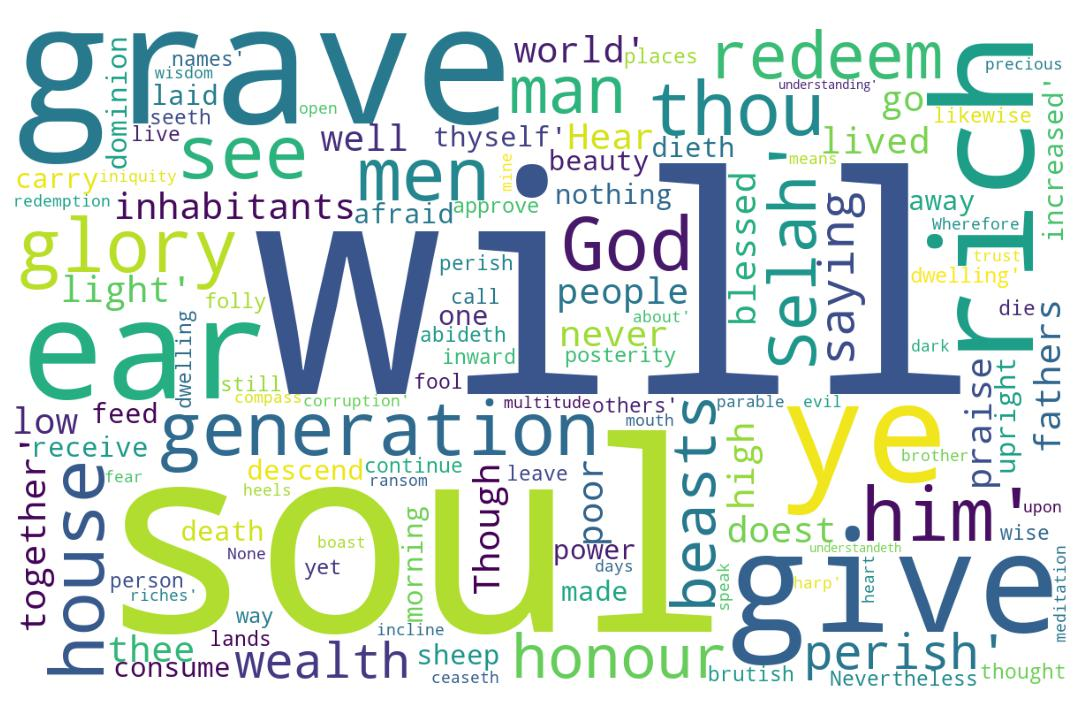
\includegraphics[width=\linewidth]{19OT-Psalms/Psalm49-WordCloud.jpg}
  \caption{Psalm 49 Word Cloud}
  \label{fig:Psalm 49 word Cloud}
\end{figure}

\marginpar{\scriptsize \centering \fcolorbox{bone}{lime}{\textbf{BIG PROBLEMS STILL REMAIN}}\\ (Psalm 49:1-20) \begin{compactenum}[I.][8]
    \item \textbf{Religious Conflict} \index[scripture]{Psalms!Psa 049:13} (Psa 49:13)
    \item \textbf{War} \index[scripture]{Psalms!Psa 049:13} (Psa 49:13)
    \item \textbf{Famine} \index[scripture]{Psalms!Psa 049:13} (Psa 49:13)
    \item \textbf{Sickness} \index[scripture]{Psalms!Psa 049:13} (Psa 49:13)
    \item \textbf{Death} \index[scripture]{Psalms!Psa 049:13} (Psa 49:13)
    \item \textbf{Natural Disasters} \index[scripture]{Psalms!Psa 049:13} (Psa 49:13)
    \item \textbf{Murder and Theft} \index[scripture]{Psalms!Psa 049:13} (Psa 49:13)
\end{compactenum}}
    
%%%%%%%%%%%%%%%%%%%%%%%%%%%%%%%%%%%%%
%%%%%%%%%%%%%%%%%%%%%%%%%%%%%%%%%%%%%
\footnote{\textcolor[cmyk]{0.99998,1,0,0}{\hyperlink{TOC}{Return to end of Table of Contents.}}}\footnote{\href{https://audiobible.com/bible/psalms_49.html}{\textcolor[cmyk]{0.99998,1,0,0}{Psalms Audio}}}\textcolor[cmyk]{0.99998,1,0,0}{To the chief Musician, A Psalm for the sons of Korah.}\footnote{This is one of the ``orphan'' psalm, with no known author (anonymous), But, it is one of eleven psalms that were for the sons of Korah. (Psalm 42, 44, 45, 46, 47, 48, 49, 84, 85, 87, and 88). The sons of Korah descended from a father who perished under the wrath and curse of God because of his arrogance and pride.   As Korah was a Levite, grandson of Kohath, great-grandson of Levi, this only aggravated his fault, and typifies the sin of Israel, keepers of the oracles of God. \cite{Phillips2001ExploringPsalms1} The count of the psalms for the sons of Korah points to the number 11 as the number of the ``remnant'' as does Hebrews 11 which lists those distinct and select people know for the exercise of faith.}\\
\\
\textcolor[cmyk]{0.99998,1,0,0}{Hear this, all \emph{ye} people; give ear, all \emph{ye} inhabitants of the world:}
[2] \textcolor[cmyk]{0.99998,1,0,0}{Both low and high, rich and poor, together.}
[3] \textcolor[cmyk]{0.99998,1,0,0}{My mouth shall speak of wisdom; and the meditation of my heart \emph{shall} \emph{be} of \fcolorbox{bone}{MYGOLD}{understanding}.}
[4] \textcolor[cmyk]{0.99998,1,0,0}{I will incline mine ear to a parable: I will open my dark saying upon the harp.}
[5] \textcolor[cmyk]{0.99998,1,0,0}{Wherefore should I fear in the days of evil, \emph{when} the iniquity of my heels shall compass me about?}\footnote{The words ``heels'' is found four times in scripture, signifying that someone’s iniquities are following them. What we have done catches up with us (vs. 5). The steps we have stepped, out run us eventually because we step slower and slower. Sooner or later they compass us round about: \cite{Ruckman1992Psalms}
\begin{compactenum}
\item \textbf{Genesis 49:17} -- Dan shall be a serpent by the way, an adder in the path, that biteth the horse heels, so that his rider shall fall backward.
\item \textbf{Job 13:27} -- Thou puttest my feet also in the stocks, and lookest narrowly unto all my paths; thou settest a print upon the heels of my feet.
\item \textbf{Psalm 49:5} -- Wherefore should I fear in the days of evil, \emph{when} the iniquity of my heels shall compass me about?
\item \textbf{Jeremiah 13:22} -- And if thou say in thine heart, Wherefore come these things upon me? For the greatness of thine iniquity are thy skirts discovered, \emph{and} thy heels made bare.
\end{compactenum} }
[6] \textcolor[cmyk]{0.99998,1,0,0}{They that trust in \fcolorbox{bone}{bone}{their} wealth, and boast themselves in the multitude of \fcolorbox{bone}{bone}{their} riches;}\marginpar{\scriptsize \textcolor[rgb]{0.00,0.545,0.269}{$\rightarrow$``Their'' things: 
\begin{compactenum}
	\item their wealth [6, 10],
	\item their riches [6],
	\item their soul [7],
	\item their inward thought [11],
	\item their houses [11],
	\item their dwelling places [11],
	\item their lands [11],
	\item their names [11],
	\item their way [13],
	\item their folly [13],
	\item their posterity [13],
	\item their sayings [13],
	\item their beauty [15], and
	\item dwelling  [15].
\end{compactenum}}}
[7] \textcolor[cmyk]{0.99998,1,0,0}{None \emph{of} \emph{them} can by any means redeem his brother, nor give to God a ransom for him:}
[8] \textcolor[cmyk]{0.99998,1,0,0}{(For the redemption of \fcolorbox{bone}{bone}{their} soul \emph{is} precious, and it ceaseth for ever:)}
[9] \textcolor[cmyk]{0.99998,1,0,0}{That he should still live for ever, \emph{and} not see corruption.}
[10] \textcolor[cmyk]{0.99998,1,0,0}{For he seeth \emph{that} wise men die, likewise the fool and the brutish person perish, and leave \fcolorbox{bone}{bone}{their} wealth to others.}
[11] \textcolor[cmyk]{0.99998,1,0,0}{Their inward thought \emph{is}, \emph{that} \fcolorbox{bone}{bone}{their} houses \emph{shall} \emph{continue} for ever, \emph{and} \fcolorbox{bone}{bone}{their} dwelling places to all generations; they call \emph{their} lands after \fcolorbox{bone}{bone}{their} own names.}
[12] \textcolor[cmyk]{0.99998,1,0,0}{Nevertheless man \emph{being} in honour abideth not: he is like the beasts \emph{that} perish.}
[13] \textcolor[cmyk]{0.99998,1,0,0}{This \fcolorbox{bone}{lime}{\fcolorbox{bone}{bone}{their} way} \emph{is} \fcolorbox{bone}{bone}{their} folly: yet \fcolorbox{bone}{bone}{their} posterity approve \fcolorbox{bone}{bone}{their} sayings. Selah.}
[14] \textcolor[cmyk]{0.99998,1,0,0}{Like sheep they are laid in the grave; death shall feed on them; and the upright shall have dominion over them in the morning; and \fcolorbox{bone}{bone}{their} beauty shall consume in the grave from \fcolorbox{bone}{bone}{their} dwelling.}
[15] \textcolor[cmyk]{0.99998,1,0,0}{But God will redeem my soul from the power of the grave: for he shall receive me. Selah.}
[16] \textcolor[cmyk]{0.99998,1,0,0}{Be not thou afraid when one is made rich, when the glory of his house is increased;}
[17] \textcolor[cmyk]{0.99998,1,0,0}{For when he dieth he shall carry nothing away: his glory shall not descend after him.}
[18] \textcolor[cmyk]{0.99998,1,0,0}{Though while he lived he blessed his soul: and \emph{men} will praise thee, when thou doest well to thyself.}
[19] \textcolor[cmyk]{0.99998,1,0,0}{He shall go to the generation of his fathers; they shall never see light.}
[20] \textcolor[cmyk]{0.99998,1,0,0}{Man \emph{that} \emph{is} in honour, and \fcolorbox{bone}{MYGOLD}{understandeth} not, is like the beasts \emph{that} perish.}

\chapter{Proverb 18}
\begin{figure}
  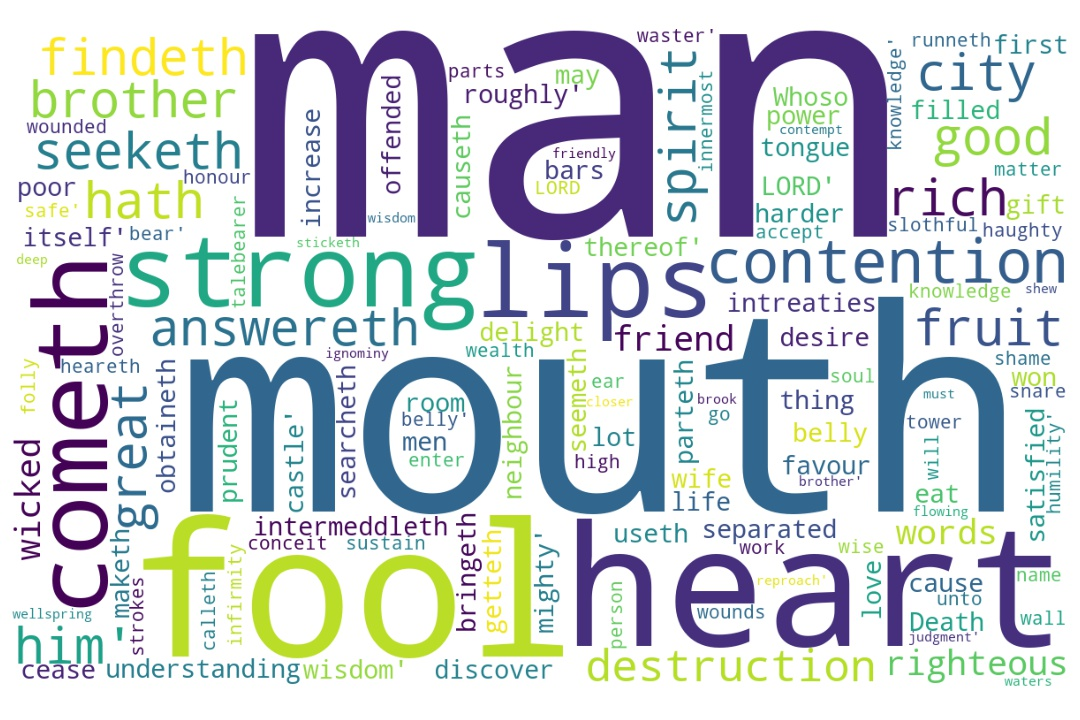
\includegraphics[width=\linewidth]{20OT-Proverbs/Proverb18-WordCloud.jpg}
  \caption{Proverb 18 Word Cloud}
  \label{fig:Proverb 18 word Cloud}
\end{figure}

\marginpar{\scriptsize \centering \fcolorbox{bone}{lime}{\textbf{A MAN FOCUSED ON GOD}}\\ (Proverbs 18:1-24) \begin{compactenum}[I.][8]
    \item Will be an \textbf{Inspired Man} - 
    \item Will be \textbf{Separate from the Ignorant Masses} - 
    \item For him most things in life will have  
    \textbf{Insignificant Meaning} - 
    \item Lives in an \textbf{Isolated Manner} 
    \item Lives by an \textbf{Individual Mandate} 
    \item Has an \textbf{intense and Insular Mentality}
\end{compactenum}}

\marginpar{\scriptsize \centering \fcolorbox{bone}{yellow}{\textbf{A FRIEND LIKE JESUS}}\\ (Proverb 18:24) \begin{compactenum}[I.][8]
    \item A \textbf{Close} Friend
    \item A \textbf{Constant} Friend
    \item A \textbf{Confiding} Friend
    \item A \textbf{Concerned} Friend
    \item A \textbf{Continuing} Friend
    \item A \textbf{Capable} Friend
    \item A \textbf{Caring} Friend
\end{compactenum}}

\marginpar{\scriptsize \centering \fcolorbox{bone}{black}{\textbf{\textcolor{white}{THE PURSUIT OF WISDOM}}}\\ (Proverb 18:24) \begin{compactenum}[I.][8]
    \item Then \textbf{Perverted} Motive -- to learn how manipulate events and circumstances. \index[scripture]{Proverbs!Pro 18:01}(Proverb 18:1)
    \item Then \textbf{Prideful} Motive -- To become exalted as wise. 
    \item Then \textbf{Public} Motive -- to be known and famous. 
    \item Then \textbf{Personal} Motive -- to achieve understanding. 
    \item Then \textbf{Practical} Motive -- to learn how live without mistakes or errors. 
    \item Then \textbf{Purposeful} Motive -- to learn navigate a specific problem. 
    \item Then \textbf{Perfect} Motive -- to learn how to live righteously before God. 
\end{compactenum}}

\marginpar{\scriptsize \centering \fcolorbox{bone}{blue}{\textbf{\textcolor{white}{WHAT YOUR SPEECH REVEALS}}}\\ (Proverb 18:4) \begin{compactenum}[I.][8]
    \item \textbf{Your Education} 
    \item \textbf{Your Excellence} 
    \item \textbf{Your Excitements} 
    \item \textbf{Your Enmity} 
    \item \textbf{Your Enemies} 
    \item \textbf{Your End} 
    \item \textbf{Your Emptiness}
    \item \textbf{Your Entanglements} 
\end{compactenum} }

\marginpar{\scriptsize \centering \fcolorbox{bone}{orange}{\textbf{THE WISE MAN}}\\ (Proverbs 18:1-24) \begin{compactenum}[I.][8]
    \item \textbf{Is Distinctive}
    \item \textbf{Is Disciplined}
    \item \textbf{Ignores Distractions}
    \item \textbf{Finds Delights in Wisdom}
    \item \textbf{Has Departed from the Common and Mundane}
    \item \textbf{Has a Distaste for Foolishness}
    \item \textbf{Is often regarded as Disturbed}
\end{compactenum} }




\footnote{\textcolor[cmyk]{0.99998,1,0,0}{\hyperlink{TOC}{Return to end of Table of Contents.}}}\footnote{\href{https://audiobible.com/bible/proverbs_18.html}{\textcolor[cmyk]{0.99998,1,0,0}{Proverbs Audio}}}\textcolor[cmyk]{0.99998,1,0,0}{Through desire a man, having separated himself, seeketh \emph{and} \fcolorbox{bone}{MYGOLD}{intermeddleth} with all wisdom.}
[2] \textcolor[cmyk]{0.99998,1,0,0}{A fool hath no delight in \fcolorbox{bone}{MYGOLD}{understanding}, but that \fcolorbox{bone}{bone}{his} heart may discover itself.}
[3] \textcolor[cmyk]{0.99998,1,0,0}{When the wicked cometh, \emph{then} cometh also contempt, and with ignominy reproach.}
[4] \textcolor[cmyk]{0.99998,1,0,0}{The words of a man's mouth \emph{are} \emph{as} deep waters, \emph{and} the wellspring of wisdom \emph{as} a flowing brook.}\footnote{\textbf{Proverb 16:22} - Understanding is a wellspring of life unto him that hath it: but the instruction of fools is folly.}
[5] \textcolor[cmyk]{0.99998,1,0,0}{\emph{It} \emph{is} not good to accept the person of the wicked, to overthrow the righteous in judgment.}
[6] \textcolor[cmyk]{0.99998,1,0,0}{A fool's lips enter into contention, and \fcolorbox{bone}{bone}{his} mouth calleth for strokes.}
[7] \textcolor[cmyk]{0.99998,1,0,0}{A fool's mouth \emph{is} \fcolorbox{bone}{bone}{his} destruction, and \fcolorbox{bone}{bone}{his} lips \emph{are} the snare of \fcolorbox{bone}{bone}{his} soul.}
[8] \textcolor[cmyk]{0.99998,1,0,0}{The words of a talebearer \emph{are} as wounds, and they go down into the innermost parts of the belly.}
[9] \textcolor[cmyk]{0.99998,1,0,0}{He also that is slothful in \fcolorbox{bone}{bone}{his} work is brother to him that is a great waster.}
[10] \textcolor[cmyk]{0.99998,1,0,0}{The name of the LORD \emph{is} a strong tower: the righteous runneth into it, and is safe.}
[11] \textcolor[cmyk]{0.99998,1,0,0}{The rich man's wealth \emph{is} \fcolorbox{bone}{bone}{his} strong city, and as an high wall in \fcolorbox{bone}{bone}{his} own conceit.}
[12] \textcolor[cmyk]{0.99998,1,0,0}{Before destruction the heart of man is haughty, and before honour \emph{is} humility.}
[13] \textcolor[cmyk]{0.99998,1,0,0}{He that answereth a matter before he heareth \emph{it}, it \emph{is} folly and shame unto him.}
[14] \textcolor[cmyk]{0.99998,1,0,0}{The spirit of a man will sustain \fcolorbox{bone}{bone}{his} infirmity; but a wounded spirit who can bear?}
[15] \textcolor[cmyk]{0.99998,1,0,0}{The heart of the prudent getteth knowledge; and the ear of the wise seeketh knowledge.}
[16] \textcolor[cmyk]{0.99998,1,0,0}{A man's gift maketh room for him, and bringeth him before great men.}
[17] \textcolor[cmyk]{0.99998,1,0,0}{\emph{He} \emph{that} \emph{is} first in \fcolorbox{bone}{bone}{his} own cause \emph{seemeth} just; but \fcolorbox{bone}{bone}{his} neighbour cometh and searcheth him.}
[18] \textcolor[cmyk]{0.99998,1,0,0}{The lot causeth contentions to cease, and parteth between the mighty.}
[19] \textcolor[cmyk]{0.99998,1,0,0}{A brother offended \emph{is} \emph{harder} \emph{to} \emph{be} \emph{won} than a strong city: and \emph{their} contentions \emph{are} like the bars of a castle.}
[20] \textcolor[cmyk]{0.99998,1,0,0}{A man's belly shall be satisfied with the fruit of \fcolorbox{bone}{bone}{his} mouth; \emph{and} with the increase of \fcolorbox{bone}{bone}{his} lips shall he be filled.}
[21] \textcolor[cmyk]{0.99998,1,0,0}{Death and life \emph{are} in the power of the tongue: and they that love it shall eat the fruit thereof.}
[22] \textcolor[cmyk]{0.99998,1,0,0}{\emph{Whoso} findeth a wife findeth a good \emph{thing}, and obtaineth favour of the LORD.}
[23] \textcolor[cmyk]{0.99998,1,0,0}{The poor useth intreaties; but the rich answereth roughly.}
[24] \textcolor[cmyk]{0.99998,1,0,0}{A man \emph{that} \emph{hath} friends must shew himself friendly: and there is a friend \emph{that} sticketh closer than a brother.}




\end{document}

